    \chapter{Results}\label{chap: results}

In this chapter the results from different test cases presented in section XX will be presented. First, we discuss the verification results to understand the capabilities and issues of the optimisation process. In the next step, we validate the code performance using different data sets. Then, we focus on tensile and shear tests with non-linear loading conditions. 
Finally, we present the results of the cyclic load cases. All studies were performed with five different initial value combinations to ensure reproducibility. In the following plots, they are numbered serially. 

% eventuell plot format noch anpassen, wie voce und RMSE plot sinnvoll einbauen?
% sind RMSE plots überhaupt notwendig bei validation?
% strain-strain plot bei verification einfügen

\section{Verification}\label{sec: verification}

In this section, the results for the verification study of the optimisation process are discussed. In this study a material with mixing ratio 6:3 was tested under normal strain loading in $xx$-direction. The strain was applied linear up to a maximum value of 20 \%. As evaluated reactions $\sigma_{xx}$, $\varepsilon_{yy}$ and $\varepsilon_{zz}$ were used. To reconstruct the optimisation history, the trends of selected quantities are presented in the following.

\begin{figure}[H]
    \centering
    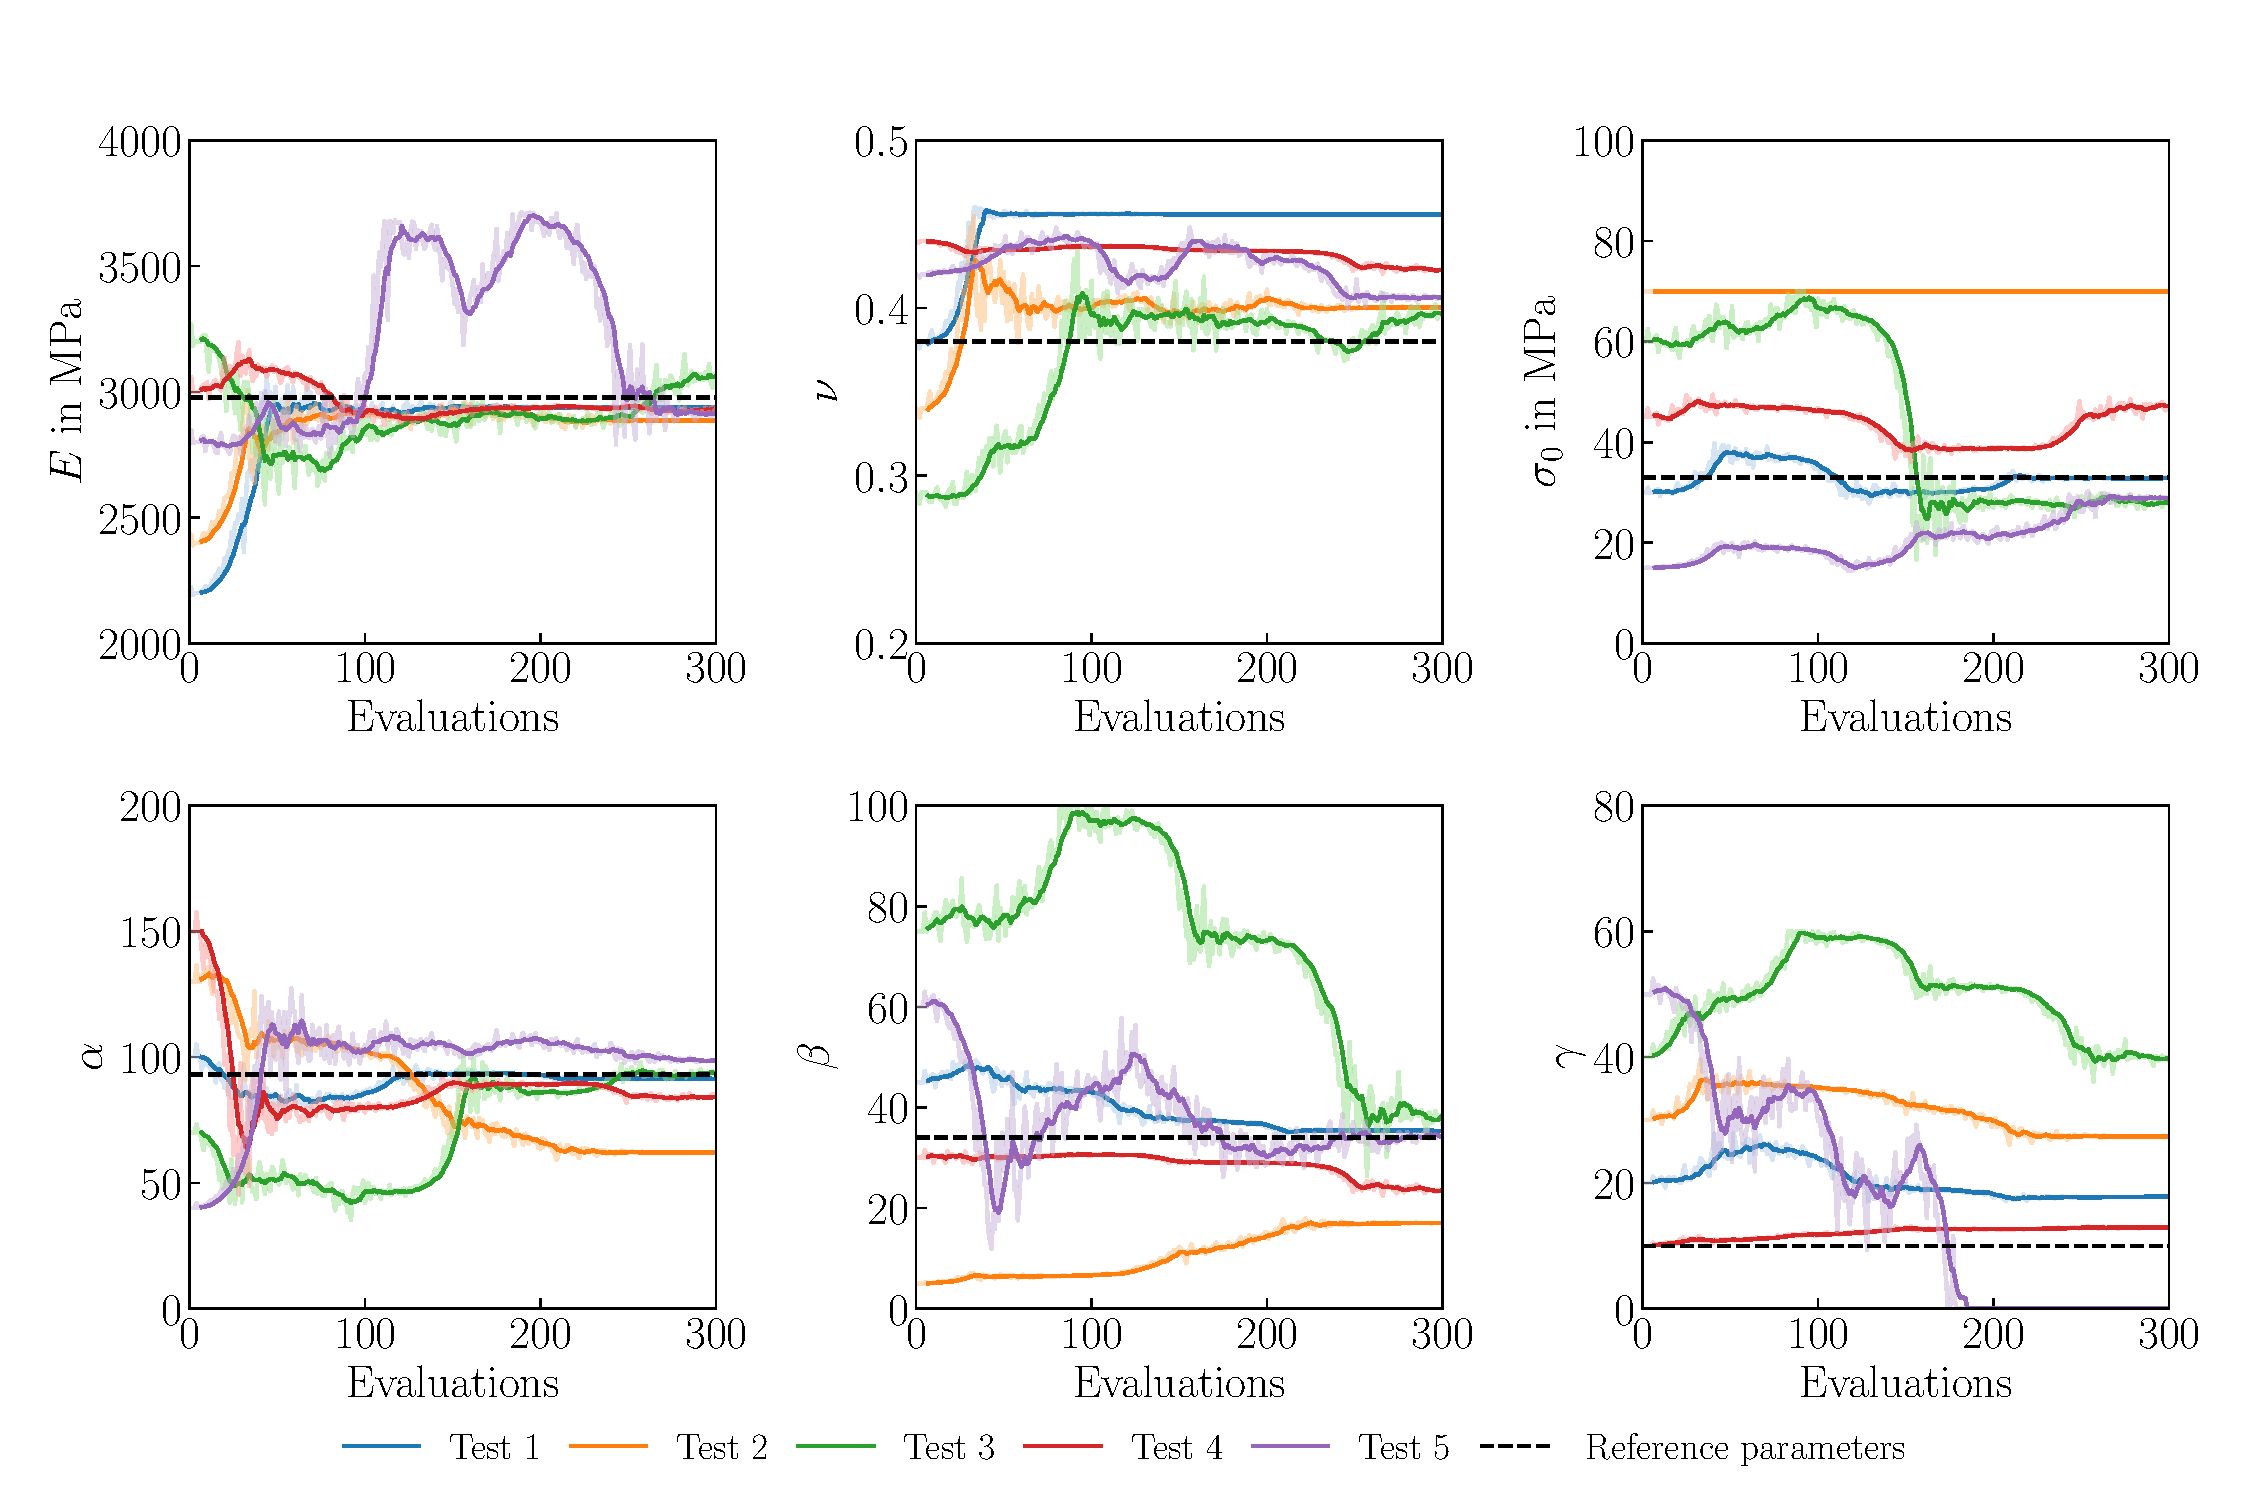
\includegraphics[width=1.0\textwidth]{Vald_6To3_Params3_material_params.pdf}
    \caption{Progress of material parameters during the verification study.}
    \label{fig:verifMaterialParams}
\end{figure}

PARAMETER JEWEILS IN ALLEN PLOTS GLEICH SKALIEREN \\


First, the material parameters are presented, since their optimisation is the main purpose of the procedure. The progress of each material parameter during the optimisation is plotted in \autoref{fig:verifMaterialParams}. The first two subplots show the elastic parameters Young's modulus $E$ and Poisson's ratio $\nu$. As explained in section XX, in the \acrshort{fem} model $C_{10}$ and $D_1$ were used as elastic parameters. However, since $E$ and $\nu$ are the more illustrative quantities, only these are represented. With \autoref{eq: elasticParams} and \ref{eq: elasticParams} the parameters can easily be converted into each other. The remaining plots show the parameters, which define the plastic hardening. It should be stated, that in all performed tests, the values of all parameters converge. Furthermore, a trend towards a certain value can be seen for all parameters except gamma. However, in all plots there is at least one outlier test. The earlier end of particular curves coheres on the internal convergence criterion of the Nelder-Mead algorithm as stated in XX.  To verify the quality of the \acrlong{omp}, the load reactions are considered. 

\begin{figure}[H]
\centering
\begin{subfigure}[t]{0.495\textwidth}
    \centering
    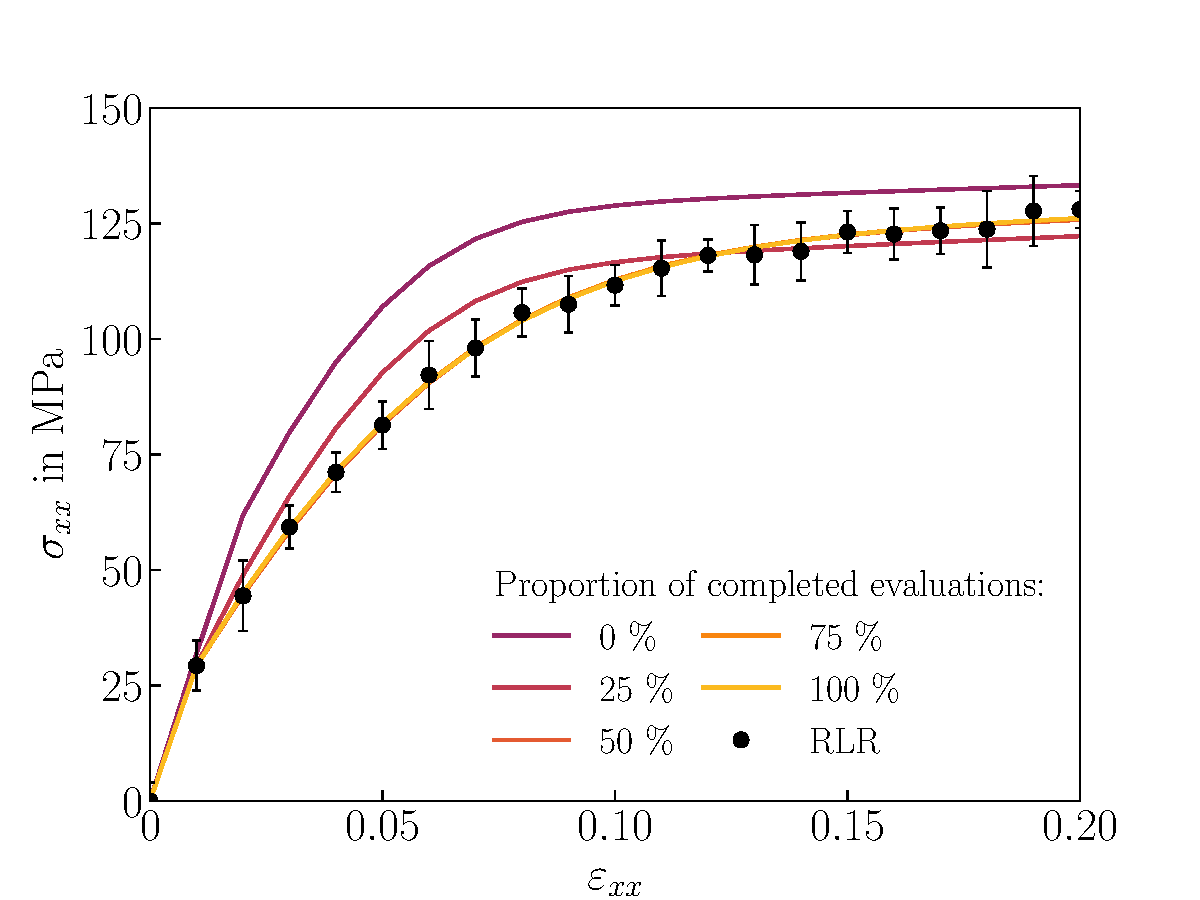
\includegraphics[width=\textwidth]{Vald_6To3_Params3_4_stress_strain_progress.pdf}
    \caption{Evolution of stress–strain curve}
    \label{fig:verifStressStrainProgress}
\end{subfigure}
\hfill
\begin{subfigure}[t]{0.495\textwidth}
    \centering
    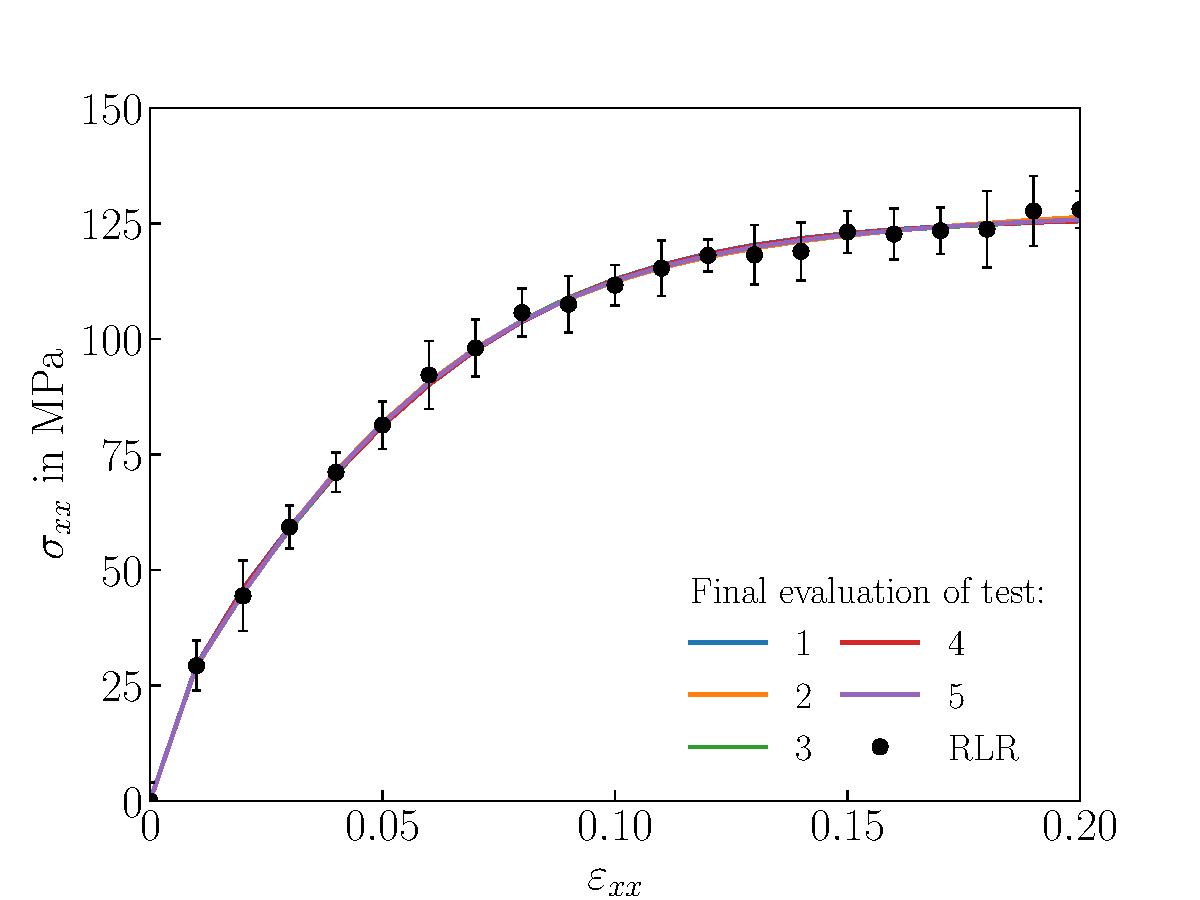
\includegraphics[width=\textwidth]{Vald_6To3_Params2_stress_strain_combined.pdf}
    \caption{Final stress–strain curves}
    \label{fig:verifStressStrainFinal}
\end{subfigure}
\caption{Verification results for load reaction $\sigma_{xx}$}
\label{fig:verifStressStrainCurves}
\end{figure}

In \autoref{fig:verifStressStrainCurves}, the load reactions $\sigma_{xx}$ are plotted against the applied strain $\varepsilon_{xx}$. The progress of the values during an exemplary test is shown in \autoref{fig:verifStressStrainProgress}. The \acrlong{rlr} are plotted as black dots with corresponding standard deviations. The \acrlong{olr} match the \acrlong{rlr} almost perfect already after 50 \% of the performed evaluations. The standard deviations are much higher than the difference between the reference points and the \acrlong{olr}. In \autoref{fig:verifStressStrainFinal} the \acrlong{olr} after the final evaluation of each test are plotted. All curves perfectly fit the points of the \acrlong{rlr}. However, $\varepsilon_{yy}$ and $\varepsilon_{zz}$ were used as \acrlong{er} as well. Because of the isotropic material behaviour, their load reactions are equal in size. Therefore, only one load reaction ($\varepsilon_{yy}$) is plotted in XX after the final evaluation. Similar, as for the stress load reactions, a high correlation between the \acrlong{olr} and the \acrlong{rlr} can be seen. The observations of all \acrlong{er} suggest that in all tests the \acrshort{rmse} was effectively reduced. To support this assumption the progress of the \acrshort{rmse} for all the tests in \autoref{fig:verifRMSEProgress}. We observe that in all tests the \acrshort{rmse} is reduced up to a limit value between 1 and 2. The value decreases quite fast in the first optimisation iterations, and then approaches slowly to its minimum value.

\begin{figure}[H]
\centering
\begin{subfigure}[t]{0.495\textwidth}
    \centering
    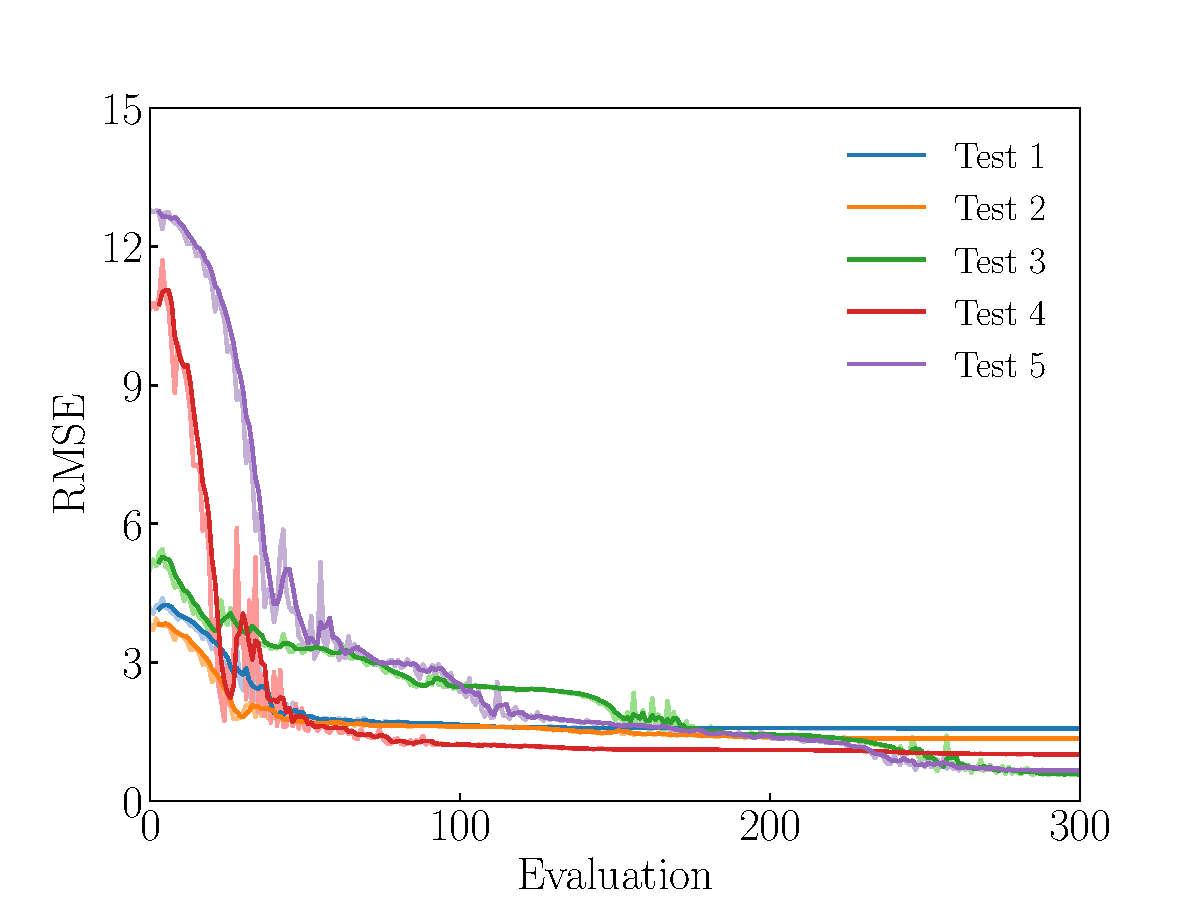
\includegraphics[width=\textwidth]{Vald_6To3_Params3_rsme_lin_plot.pdf}
    \caption{rmse for multiple tests}
    \label{fig:verifRMSEProgress}
\end{subfigure}
\hfill
\begin{subfigure}[t]{0.495\textwidth}
    \centering
    \centering
    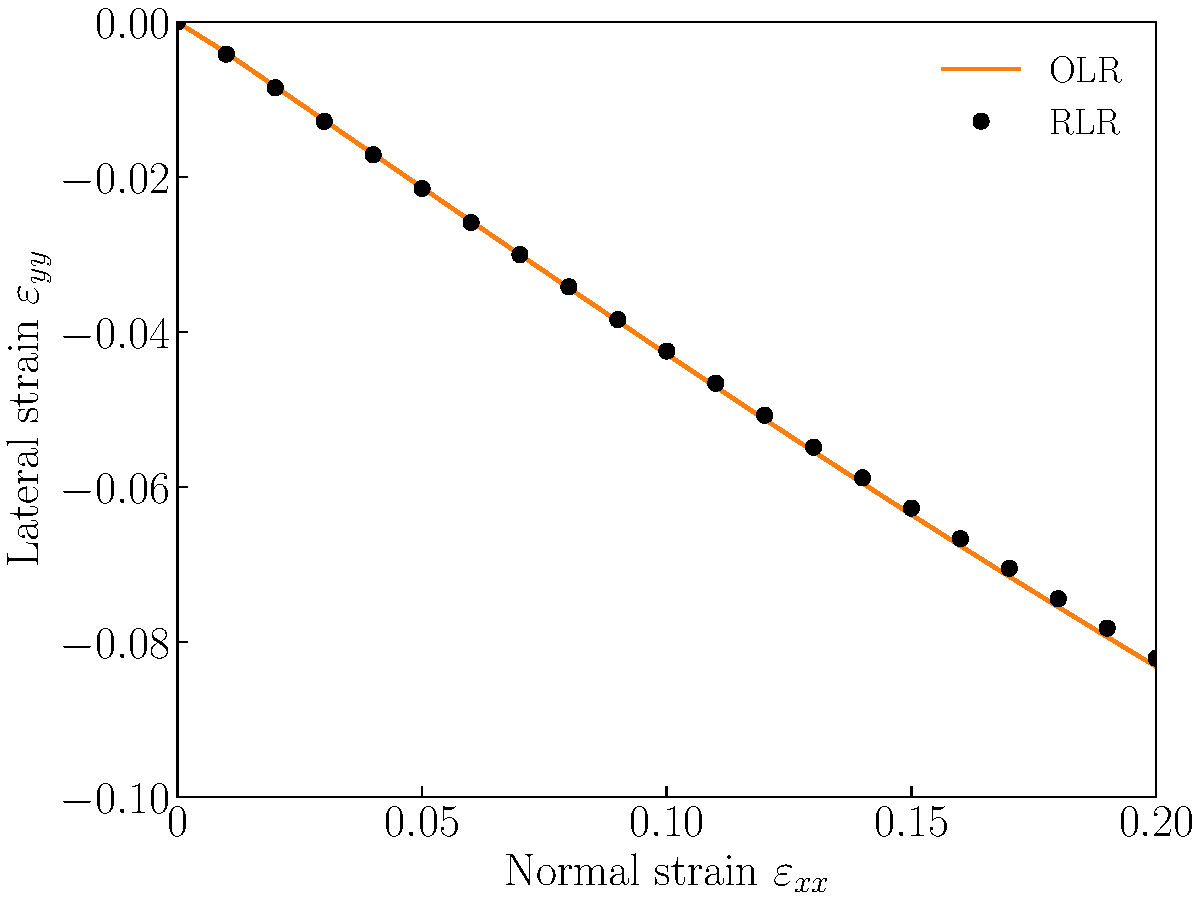
\includegraphics[width=\textwidth]{Vald_6to3_Params3_strain_strain.pdf}
    \caption{strain strain plot}
    \label{fig:verfiStrainStrain}
\end{subfigure}
\caption{Verification results for load reaction $\sigma_{xx}$}
\label{fig:voceAndRMSEVerif}
\end{figure}

\paragraph{Discussion}
The results of the \acrlong{olr} presented in Figure XX bis XX indicate an effective error reduction of the script for all tests. Independent of the initial value combination, equally high correlation levels are reached. On the contrary, the \acrlong{omp} demonstrate ambiguous values, which implies issues in finding a unique minimum. These results illustrate, that multiple \acrlong{omp} yield equal load reactions. To understand this phenomenon, the impact of the material parameters on the load reactions are analysed in detail. As described in \autoref{subsec:loadParameters}, the most load steps are placed in the plastic domain of the material, which is known from further investigations (QUELLE). Only the first load step represents elastic behaviour. Therefore, the focus is taken on the plastic parameters. Via the VOCE-hardening (\autoref{eq: voce}) the stress load reaction $\sigma_{xx}$ can be computed as a funciton of the plastic material parameters.
In \autoref{fig:voceCurve} an exemplary trend of the VOCE-function is plotted with arbitrary chosen values for the plastic parameters. The impact of each parameter on the curve is mapped by adjusting its value sequentially. The plastic yield $\sigma_0$ stays constant, since it only acts as an offset value, which influences the point at which the material starts to plastify. The parameter $\alpha$ has the greatest impact on the shape of the curve, while a variety of \(50\%\) in the parameter $\gamma$ has hardly any visible effect. The small influence of $\gamma$ explains its high variance in \autoref{fig:verifMaterialParams}. In general, the plot indicates a high flexibility in adjusting the shape of the curve through different value combinations. This consideration verifies the assumption, that various material parameter combinations lead to similar load reactions. \\

COMPARISON WITH GUNNARS DATA

\begin{figure}[H]
    \centering
    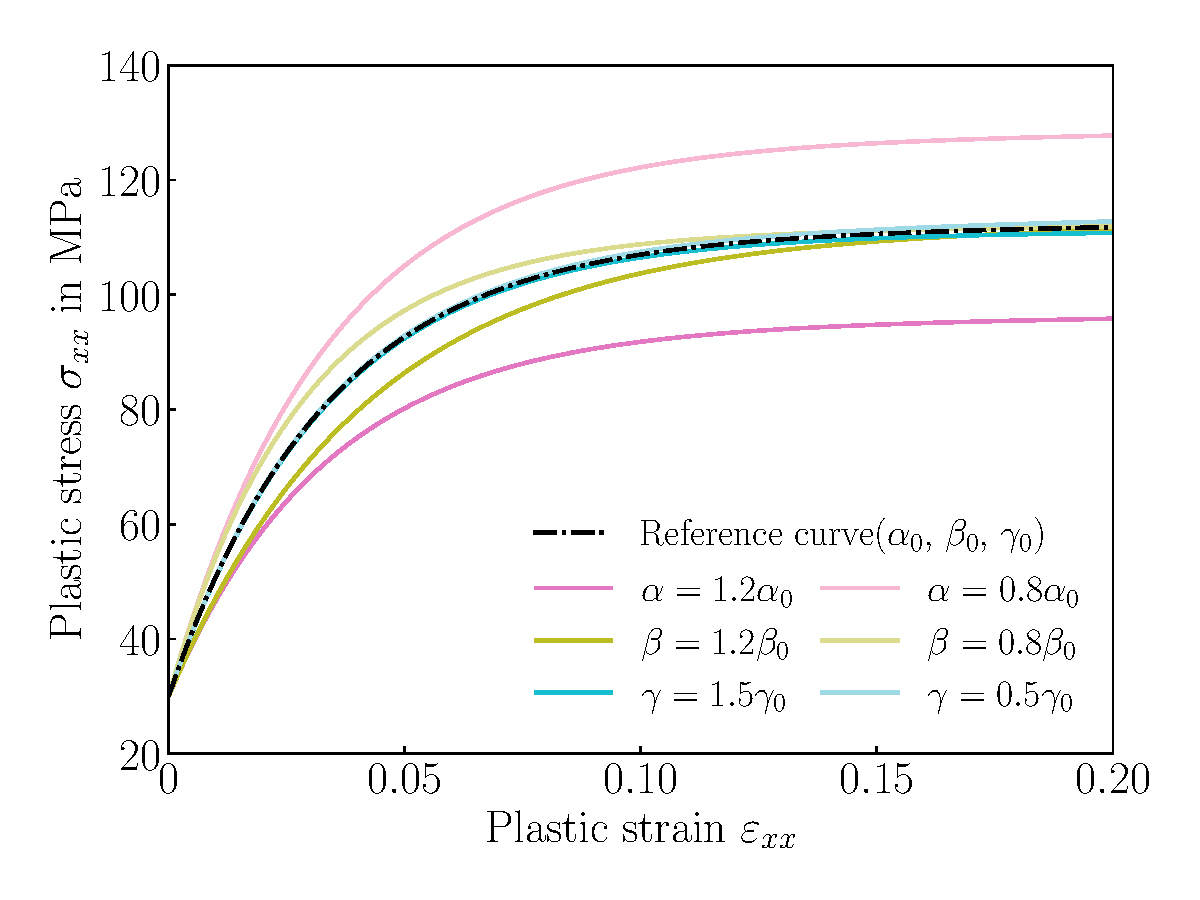
\includegraphics[width=0.5\textwidth]{voce_curve.pdf}
    \caption{parameter influence on voce-hardening curve}
    \label{fig:voceCurve}
\end{figure}

%\paragraph{Conclusion}
The presented results show, that the optimisation process generally works. It is able to reduce the error of the load reactions within an adequate number of function evaluations. However, the code is unable to find unique material parameters. To improve this, the solution space is decreased. As already stated, the elastic parameters affect only the first load step. Thus, it is possible to compute their values directly via

\begin{gather}\label{eq: EandNu}
    E = \frac{\Delta\sigma_{xx_1}}{\Delta\varepsilon_{xx_1}} \hspace{1.5cm}
    \nu = \frac{\Delta\varepsilon_{yy_1}}{\Delta\varepsilon_{xx_1}}
\end{gather}
    
Then, only the plastic material parameters need to be optimised. By adapting the process in this way, the optimisation should lead to unique values for the remaining material parameters. In the validation study this configuration is tested for material with mixing ratios 4:3, 6:3 and 8:3. \\


% To combine these observations, a detailed investigation of the 


% a common minimum  value is reached in all optimisation runs, indicating that the results are of equivalent quality. 


% Despite the high variance of the final material parameters, the stress-strain curves all matches the target data for the stress-strain curve in normal direction. Because of this deviation we depicted the influence of the parameters on the trend of the VOCE-hardening curve shown in \autoref{fig:Parameter influence on VOCE-hardening curve}.  This leads to a high flexibility in adjusting the shape of the curve and as a consequence to multiple possible parameter combinations to fit the target curve. 









% For all parameters a state of convergence is reached independent of the initial value combination. 

% However, the resulting values for one parameter differ for different tests. 


%     In the first row the elastic material parameters are presented. For a better understanding, we transformed the hyper-elastic parameters \(C10\) and \(D1\) into Young's modulus \(E\) and Poisson ratio \(\nu\). In the second row the plastic material parameters are presented. For elastic and plastic parameters we can observe convergence for every parameter combination. However, the converged solutions differ from each other for most of the combinations. 
% For a detailed discussion of possible reasons we separate between elastic and plastic material behavior. Since our tested material shows an elastic response only up to the second data point, there might be not enough optimisation points to find an unique solution for the elastic material parameters. Nevertheless, we have to investigate other characteristic quantities to ensure our assumption and understand the influence of the plastic parameters. In \autoref{fig:progress stress-strain curve} the progress of the stress-strain curve in normal direction during one exemplary test together with the target curve from the MD simulation is presented. The optimised curve matches the target curve after only  \(25 \%\) of the evaluations. Since the stress-strain curve is one of our target data this progress indicates a correct optimisation behavior of our algorithm. To support this assumption the final stress-strain curves of the test series are depicted in \autoref{fig:final stress-strain curves}. 




% The results of this verification tests lead to some states about the quality of the optimisation algorithm. The results of the stress-strain data show a good match of the optimised curve with the target data for every test which is confirmed by the RMSE. In contrast we observe a high variance in final the material parameters found by the algorithm. These results suggest that the algorithm can generally find parameter values to match the target data. However, the variance in these optimal parameters shows that multiple parameter combinations lead to the same quality of result. This behavior may be due to the relatively large number of optimisation parameters compared to the dimension of the target data. To verify this assumption we reduced the number of material parameters. Since only the first point of the target data lies in the elastic domain, we fixed the elastic material behavior and computed them directly from the data of the first point. Then we tested this new configuration of the algorithm with the current target data and two other data sets.




\newpage
\section{Validation}\label{sec: validation}
 In the validation study the elastic parameters $E$ and $\nu$ were fixed. The results of this implementation for three different data sets will be discussed in this section.
\paragraph{Test series 6:3}
In the first test series, the same material as in \autoref{sec: verification}, with mixing ratio 6:3, is used. According to \autoref{eq: EandNu} the elastic parameters are determined to 
\begin{equation*}
    E = 2916\unit{MPa} \hspace{1.5cm} \nu = 0.41 
\end{equation*}

\begin{figure}[H]
    \centering
    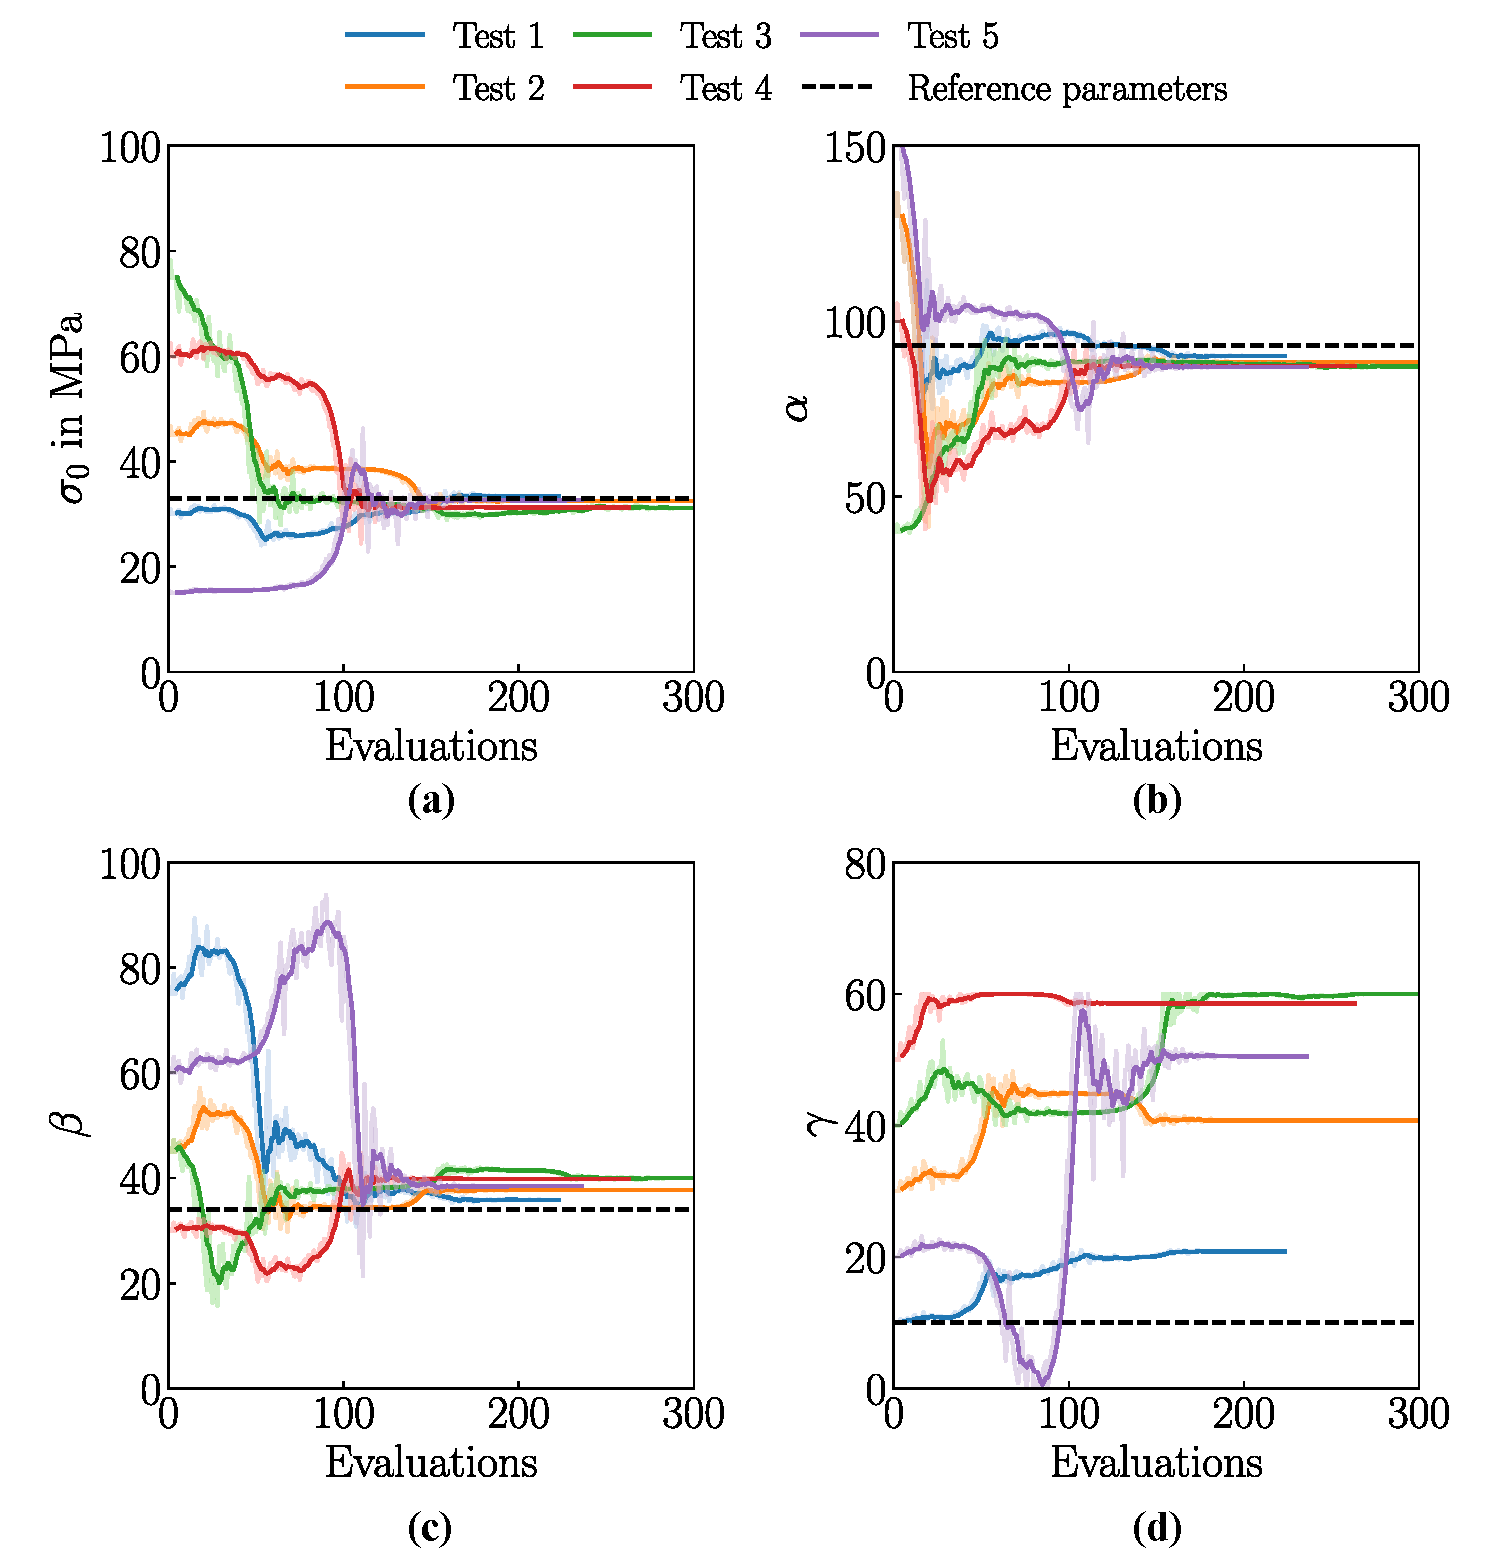
\includegraphics[width=0.7\textwidth]{Vald_6To3_fixEP1_material_params.pdf}
    \caption{progress of material parameters for validation tests}
    \label{fig:validation material params 6to3}
\end{figure}

The optimised plastic material parameters are shown in \autoref{fig:validation material params 6to3}.  In all tests, the values of $\sigma_0$, $\alpha$ and $\beta$ demonstrate a converging trend towards a singular value. Just for $\gamma$ the converged values vary for each individual test. Similar to the verification study, the quality of the \acrlong{omp} is verified by the \acrlong{olr}. In \autoref{fig:validStressStrain6to3} the final \acrlong{olr} $\sigma_{xx}$ for all tests are plotted. The curves of all tests show a perfect match of the \acrlong{rlr}. The results of the \acrlong{eer} $\varepsilon_{yy}$ and $\varepsilon_{zz}$ are added in Attachment XX, since their presentation would be beyond the scope of this work. It can be stated, that in all tests the \acrlong{olr} match the \acrlong{rlr} of the lateral strains. Their influence on the optimisation is implicitly included in the \acrshort{rmse}, which is depicted in \autoref{fig:validRMSE6to3}. Similar to the verification study, the \acrshort{rmse} decreases rapidly in the beginning, and then holds a minimum value until the test is finished.


% The quality of this optimised parameters is ensured through the match of the stress-strain curves with the target data. As demonstrated in \autoref{fig:validStressStrain6to3} the final stress-strain curves exhibit a strong correlation with the target data. The evolution of the RMSE XXX supports this results with small values for every test. A comparison of the results of the present study with those of the verification study reveals an equivalent level of optimisation quality. Additionally, the results of the material parameters indicate a positive impact of the algorithm modification, showing a unique solution for the important parameters. 

\begin{figure}[H]
\centering
\begin{subfigure}[t]{0.495\textwidth}
    \centering
    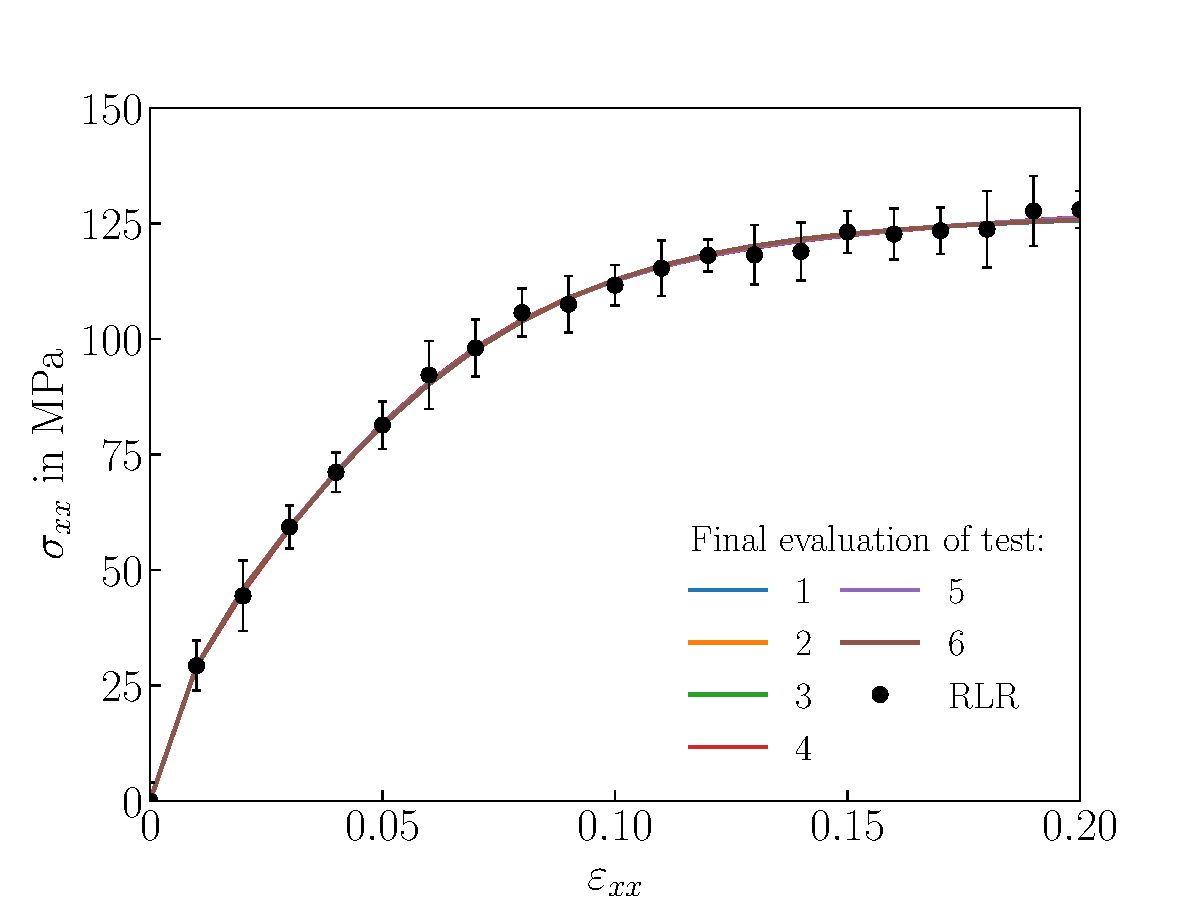
\includegraphics[width=\textwidth]{Vald_6To3_fixEP1_stress_strain_combined.pdf}
    \caption{ Final stress-strain curves}
    \label{fig:validStressStrain6to3}
\end{subfigure}
\hfill
\begin{subfigure}[t]{0.495\textwidth}
    \centering
    \centering
    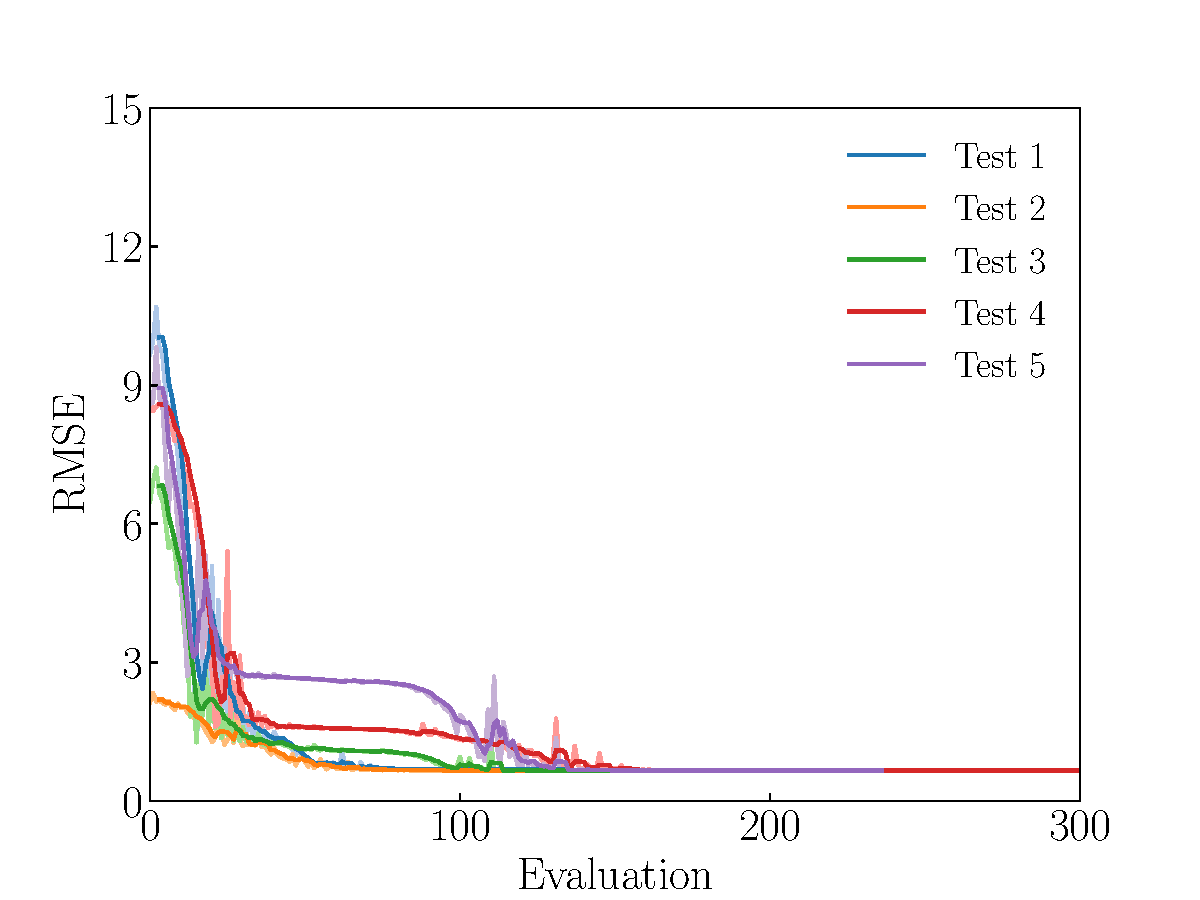
\includegraphics[width=\textwidth]{Vald_6To3_fixEP1_rsme_lin_plot.pdf}
    \caption{RMSE evolution}
    \label{fig:validRMSE6to3}
\end{subfigure}
\caption{Verification results for load reaction $\sigma_{xx}$}
\label{fig:validRes6to3}
\end{figure}




% As was outlined in the preceding discussion, gamma exerts minimal influence on the trend of the hardening curve. Consequently, the focus shall be directed towards the plastic yield, alpha and beta, which indicate an improvement in their optimisation behavior.

\paragraph{Test series 4:3 and 8:3}
In the following the results from the validation studies for materials with mixing ratio 4:3 and 8:3 are presented. The results of these two test series are discussed together, since their results lead to similar conclusions. In addition, the discussions of the \acrlong{omp} and the \acrshort{rmse} are reduced on the final values. Since these two validation series focus on the improvement of the final values of \acrlong{omp}, no relevant information is neglected through this diminution. The corresponding evolution plots are added in Attachment XX. The plastic material parameters and the \acrshort{rmse} show the same trends for both mixing ratios as for the mixing ratio 6:3. The final values of the plastic material parameters and the \acrshort{rmse} are summarised in \autoref{tab:validMaterialParams4To3} and \autoref{tab:validMaterialParams8To3}. The fixed elastic parameters are included as well. 
For both mixing ratios, the values for the material parameters were determined within a small range of variation for all tests. Only the parameter $\gamma$ shows high variations between each test. The \acrshort{rmse} reaches in all test an equally low value. Finally, the \acrlong{olr} $\sigma_{xx}$ are evaluated in \autoref{fig:validStressStrain4and8}. It represents a high correlation of all tests with its corresponding \acrlong{rlr}.

\begin{table}[h!]
\centering
\caption{Extracted material parameters for mixing ratio 4:3}
\label{tab:validMaterialParams4To3}
\renewcommand{\arraystretch}{1.2}
\begin{tabular}{L{0.08\textwidth}|C{0.08\textwidth}C{0.08\textwidth}C{0.08\textwidth}C{0.08\textwidth}C{0.08\textwidth}C{0.08\textwidth}C{0.08\textwidth}}
\toprule
\textbf{Test} & \textbf{E (MPa)} & $\boldsymbol{\nu}$ & $\boldsymbol{\sigma_0}$ \textbf{(MPa)} & $\boldsymbol{\alpha}$ & $\boldsymbol{\beta}$ & $\boldsymbol{\gamma}$ & \textbf{\acrshort{rmse}}\\
\midrule
1 & 2478 & 0.43 & 28.48 & 66.97 & 50.54 & 45.74 & 0.68 \\
2 & 2478 & 0.43 & 30.60 & 68.21 & 44.95 & 17.99 & 0.70 \\
3 & 2478 & 0.43 & 30.89 & 68.40 & 44.31 & 13.80 & 0.70 \\
4 & 2478& 0.43 & 31.37 & 68.01 & 43.97 & 13.25 & 0.70 \\
5 & 2478 & 0.43 & 30.03 & 67.99 & 46.39 & 23.78 & 0.69 \\
\bottomrule
\end{tabular}
\end{table}

\begin{table}[h!]
\centering
\caption{Extracted material parameters with RMSE values for mixing ratio 8:3}
\label{tab:validMaterialParams8To3}
\renewcommand{\arraystretch}{1.2}
\begin{tabular}{L{0.08\textwidth}|C{0.08\textwidth}C{0.08\textwidth}C{0.08\textwidth}C{0.08\textwidth}C{0.08\textwidth}C{0.08\textwidth}C{0.08\textwidth}}
\toprule
\textbf{Test} & \textbf{E (MPa)} & $\boldsymbol{\nu}$ & $\boldsymbol{\sigma_0}$ \textbf{(MPa)} & $\boldsymbol{\alpha}$ & $\boldsymbol{\beta}$ & $\boldsymbol{\gamma}$ & \textbf{\acrshort{rmse}}\\
\midrule
1 & 2636 & 0.42 & 44.45 & 60.27 & 51.33 & 60.00 & 0.58 \\
2 & 2636 & 0.42 & 46.39 & 63.09 & 43.52 & 20.25 & 0.61 \\
3 & 2636 & 0.42 & 46.69 & 64.12 & 41.94 & 9.06 & 0.62 \\
4 & 2636 & 0.42 & 44.45 & 60.26 & 51.32 & 60.00 & 0.58 \\
5 & 2636 & 0.42 & 45.97 & 61.62 & 46.00 & 35.83 & 0.60 \\
\bottomrule
\end{tabular}
\end{table}




% The evolution of the plastic material parameters for the mixing ratios 4:3 and 8:3 in plotted in \autoref{fig:validation material params}. We can observe a similar convergence behaviour as in the validation study with mixing ratio 6:3. Only test case 3 for mixing ratio 8:3 shows a deviation provided that all values converge quite late. Since we chose the initial values randomly this might occur through an unfavourable combination of values. 
% In \autoref{fig:validation results} we represent the optimised stress-strain curves and the evolution of the RMSE. For all tests the stress-strain values correlate with the target data. The equivalent level of the RMSE for the converged solutions indicate a similar quality of the optimisation result for all tests. These results indicate an improvement of the solution results through determining the elastic parameters.

\begin{figure}[H]
\centering

% --- obere Reihe: 4:3 ---
\begin{subfigure}[t]{0.495\textwidth}
    \centering
    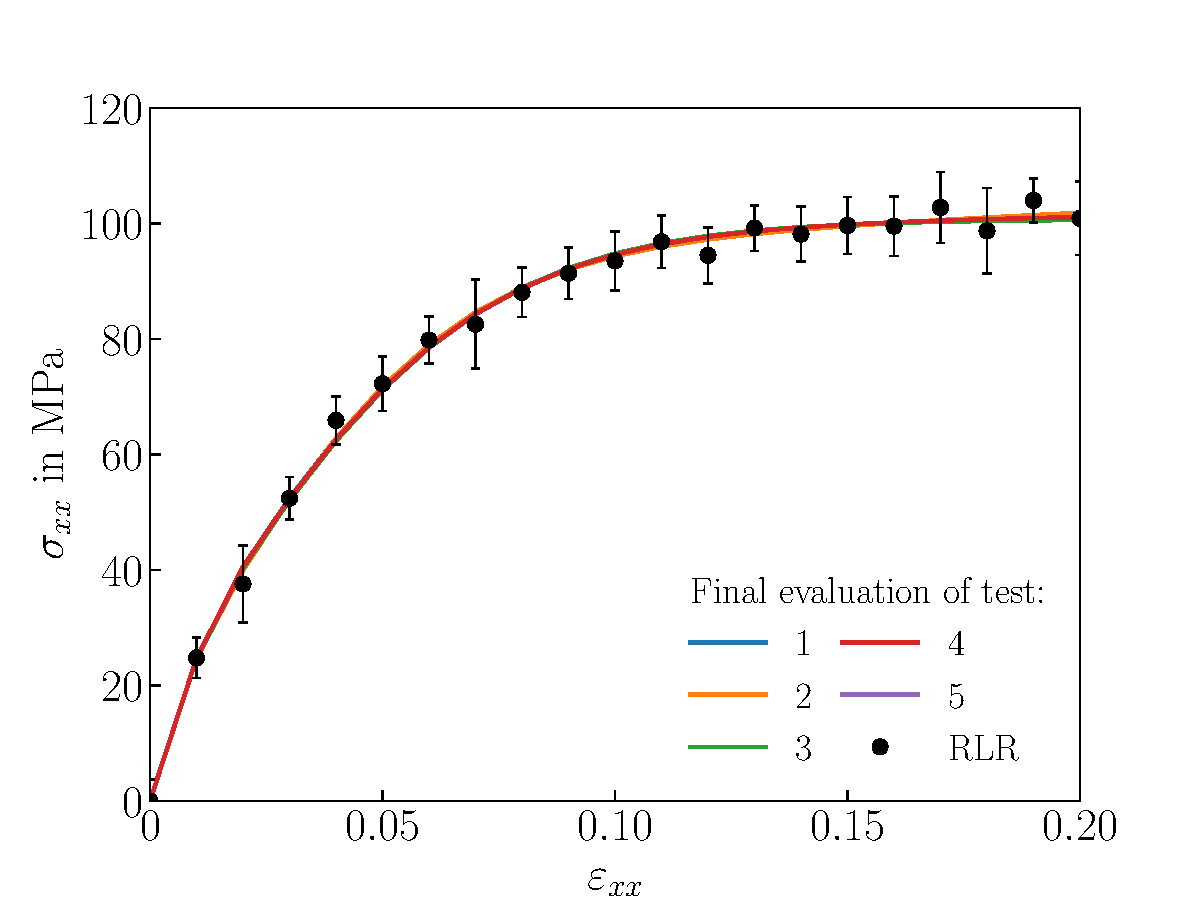
\includegraphics[width=\textwidth]{Vald_4To3_fixEP1_stress_strain_combined.pdf}
    \caption{Stress–strain curves (4:3)}
    \label{fig:validStressStrain4to3}
\end{subfigure}
\hfill
\begin{subfigure}[t]{0.495\textwidth}
    \centering
    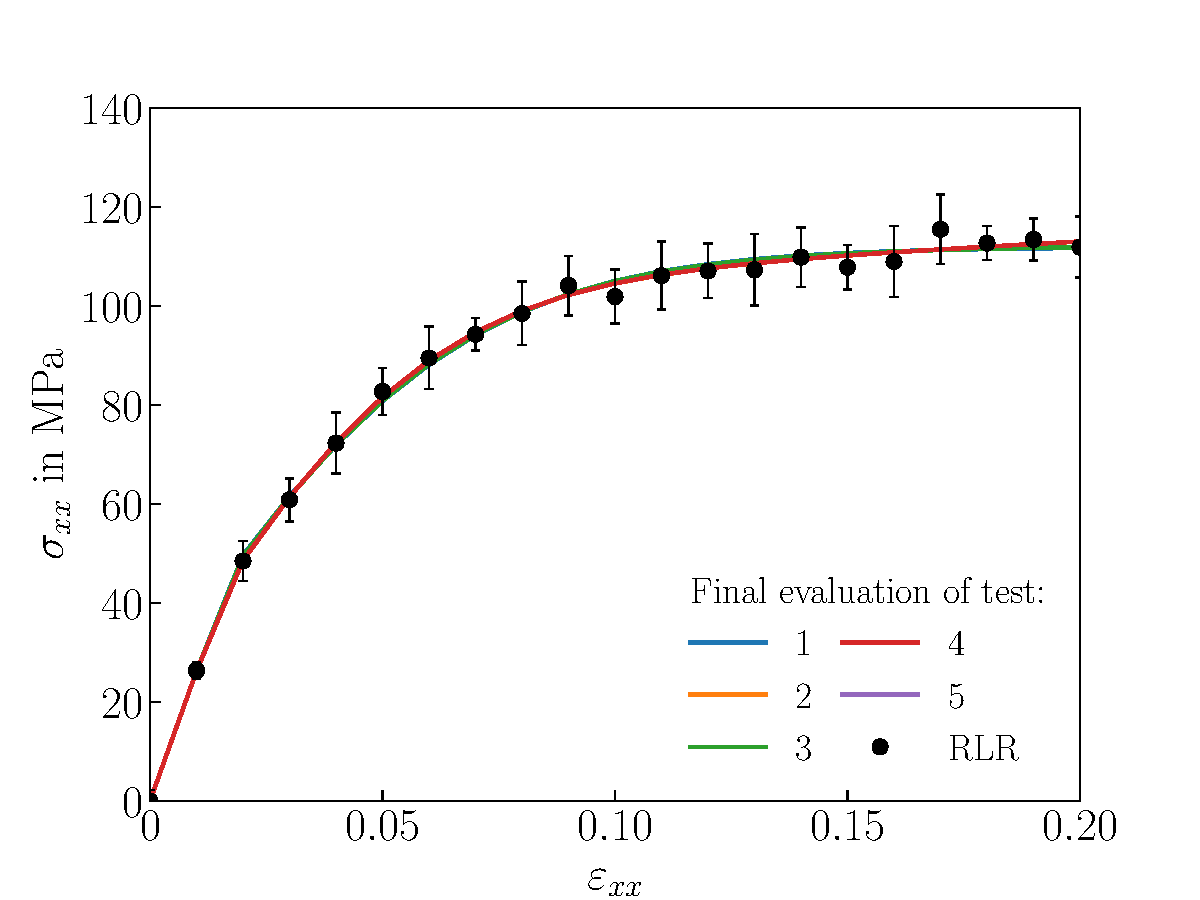
\includegraphics[width=\textwidth]{Vald_8To3_fixEP1_stress_strain_combined.pdf}
    \caption{Stress–strain curves (8:3)}
    \label{fig:validStressStrain8to3}
\end{subfigure}
\caption{Results of validation tests with mixing ratios 4:3 and 8:3:}
\label{fig:validStressStrain4and8}
\end{figure}


\paragraph{Discussion}
The performed validation studies demonstrate an improved convergence behaviour of the optimisation. For all mixing ratios, unique values for the parameters $\sigma_0$, $\alpha$ and $\beta$ are determined, independent of the initial value combination. The value of $\gamma$ still varies in a wide range. However, the impact of $\gamma$ on the trend of the hardening curve is relatively small as demonstrated in \autoref{fig:voceCurve}. Therefore, its unique definition is challenging. The \acrshort{rmse} and the stress load reactions ensure a high correlation to the \acrlong{rlr}. These results improve the reliability of the developed optimisation script. Overall, it can be stated that for a single linear applied load case with fixed elastic parameters, the script is able to find unique plastic parameters which appropriately match the material behaviour.


% Overall, these results demonstrate the reliability of the optimisation algorithm for the load case of a single tensile strain in one direction with fixed elastic parameters. The specification of the elastic parameter values improves the optimisation performance in a way, that the plastic yield $\sigma_0$, $\alpha$ and $\beta$ can be 

% However, the manual specification of Youngs modulus and Poisson ratio is only possible for target data sets with exactly one data point in the elastic domain of the material. For data sets with multiple points in the elastic domain a manual specification becomes complicated quite fast. Additional, for materials with completely unknown material behaviour, the point of transition between elastic and plastic behaviour is still unknown. In order to process such data sets too, we need to integrate the elastic parameters in the optimisation process. In doing so the singularity of the solution should be maintained. Therefore the algorithm needs additional information about the mechanical material behaviour. In the following step we tried to do so through the combination of two load cases. Additional to the already tested tensile strain we applied a shear strain. As described in section XX the shear modulus contains information about Youngs modulus and  Poisson ratio what might improve the performance of the optimisatoin process. The information contained within the shear modulus about Youngs modulus and Poisson ratio might enclose the necessary restrictions to reduce the solution variability. 

% Warum sinusförmige belastung? Jz schon mit zyklischen versuchen kommen?


\section{Tensile-Shear combination}
In this section the optimisation results for sinusoidal load application are presented. Similar to the validation studies, we calculated the elastic parameters previously with the first stress-strain data. First a tensile strain  XX is applied with the load case E11. In the second test series the same load parameters are adapted as shear load case G12, and finally, the load cases are combined in a single optimisation. In all test series, mixing ratio 6:3 was simulated. The load parameters follow the first quarter of a sinus function up to a maximum amplitude of 15 \%. 

\paragraph{Tensile tests}
In the first test series, a single tensile load case is applied. Similar as in the last validation studies, we focus on the final results of the script. Therefore, the material parameters from the final evaluation are summarised in \autoref{tab:tensileMatparams}. All tests lead to unique values for the plastic yield, alpha and beta. The values of gamma show high variances. 

\begin{table}[h!]
\centering
\caption{Extracted material parameters with RMSE values (rounded to two decimals)}
\label{tab:tensileMatparams}
\renewcommand{\arraystretch}{1.1}
\begin{tabular}{L{0.08\textwidth}|C{0.08\textwidth}C{0.08\textwidth}C{0.08\textwidth}C{0.08\textwidth}C{0.08\textwidth}C{0.08\textwidth}}
\toprule
\textbf{Test} & \textbf{E (MPa)} & $\boldsymbol{\nu}$ & $\boldsymbol{\sigma_0}$ \textbf{(MPa)} & $\boldsymbol{\alpha}$ & $\boldsymbol{\beta}$ & $\boldsymbol{\gamma}$ \\
\midrule
202 & 2599 & 0.42 & 45.50 & 78.14 & 31.23 & 55.46  \\
283 & 2599 & 0.42 & 46.37 & 84.24 & 28.15 & 0.00 \\
365 & 2599 & 0.42 & 45.47 & 77.64 & 31.49 & 59.95 \\
132 & 2599 & 0.42 & 46.61 & 82.87 & 28.31 & 10.97 \\
183 & 2599 & 0.42 & 46.07 & 81.84 & 29.18 & 22.11 \\
\bottomrule
\end{tabular}
\end{table}

To classify the results, the load reactions $\sigma_{xx}$ and the \acrshort{rmse} value are plotted in \autoref{fig:tensileResults6to3}. The \acrlong{olr} show a high correlation to the \acrlong{rlr}. We have deliberately omitted the standard deviations in this plot, as this would otherwise reduce clarity. The \acrshort{rmse} starts at quite high values,c ompared to the ones in the validation studies. However, the value decreases fast after the first evaluations, and convergences to a limit value around 2. 

\begin{figure}[H]
\centering
\begin{subfigure}[t]{0.495\textwidth}
    \centering
    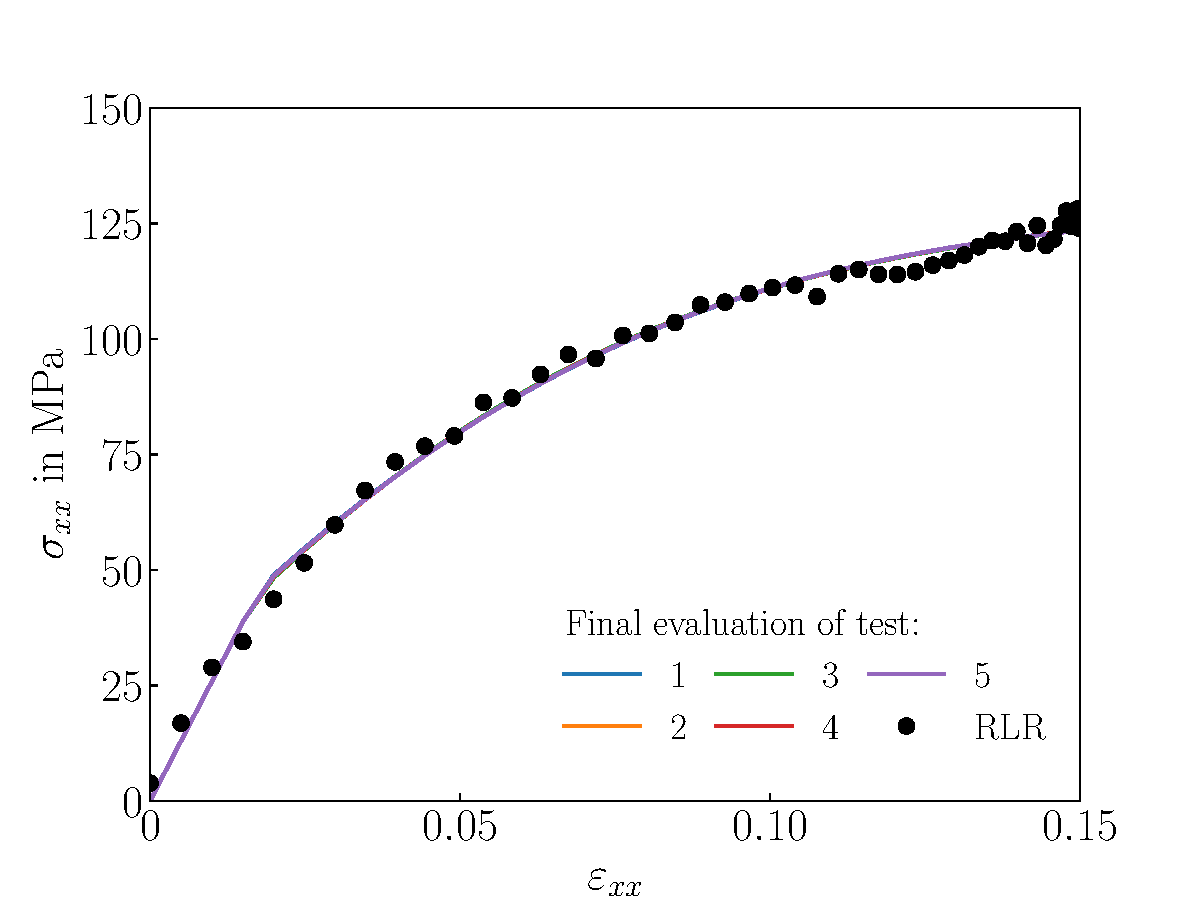
\includegraphics[width=\textwidth]{Tensile_6to3_015_fixENu_normal_stress_strain_combined.pdf}
    \caption{Final tensile stress-strain curves}
    \label{fig:tensileStressStrain6to3}
\end{subfigure}
\hfill
\begin{subfigure}[t]{0.495\textwidth}
    \centering
    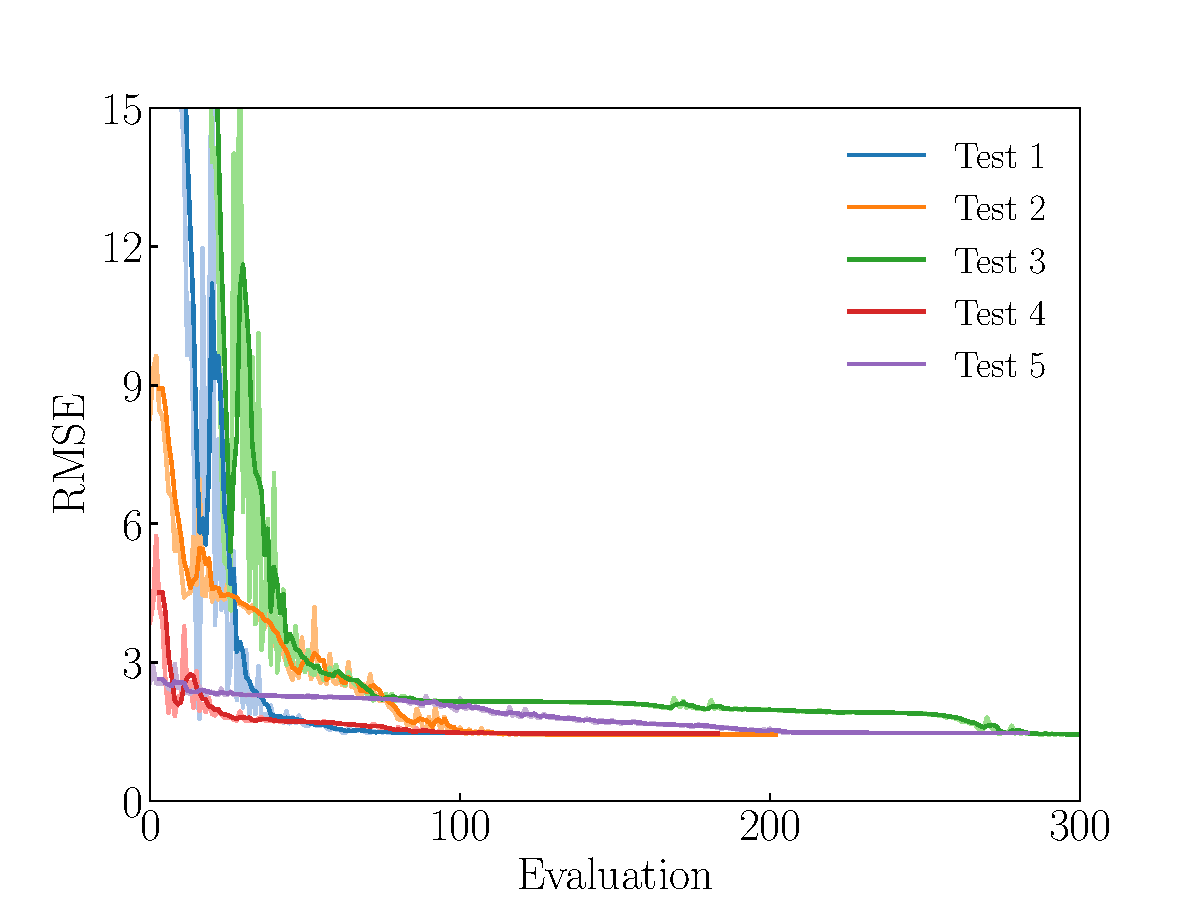
\includegraphics[width=\textwidth]{Tensile_6to3_015_fixENu_rsme_lin_plot.pdf}
    \caption{RMSE evolution}
    \label{subfigure:tensileRMSE}
\end{subfigure}
\caption{Results of tensile tests with 6to3 dataset}
\label{fig:tensileResults6to3}
\end{figure}



\paragraph{Shear tests}
In the next test series, a single shear strain is applied. The computation of the elastic parameters, needs to be adapted, since the Young's modulus cannot be computed directly. From the shear stress, we first calculate the shear modulus $G$ with the following formula
\begin{equation}
    G = \frac{\Delta\sigma_{xy}}{2\Delta\varepsilon_{xy}} = 1619\unit{MPa}
\end{equation}
which can be transferred into $E$ through
\begin{equation}
    E = 2G(1+\nu) 
\end{equation}
We chose the value of $\nu$ in a way, that the resulting Young's modulus is XXX. The final values for all material parameters are listed in \autoref{tab:shearMatParams}. In this study, the value of $\sigma_0$ ran into the limits in every test, since the upper limit is 50 MPa and the lower limit 15 MPa. For gamma the limits of 0  and 100 are reached as well. For $\alpha$ and $\beta$ similar values are reached for all tests except test number 2. 

\begin{table}[h!]
\centering
\caption{Extracted material parameters with RMSE values (rounded to two decimals)}
\label{tab:shearMatParams}
\renewcommand{\arraystretch}{1.1}
\begin{tabular}{L{0.08\textwidth}|C{0.08\textwidth}C{0.08\textwidth}C{0.08\textwidth}C{0.08\textwidth}C{0.08\textwidth}C{0.08\textwidth}}
\toprule
\textbf{Test} & \textbf{E (\unit{MPa})} & $\boldsymbol{\nu}$ & $\boldsymbol{\sigma_0}$ \textbf{(MPa)} & $\boldsymbol{\alpha}$ & $\boldsymbol{\beta}$ & $\boldsymbol{\gamma}$ \\
\midrule
311 & 4402 & 0.36 & 15.00 & 103.41 & 128.88 & 100.00 \\
241 & 4402 & 0.36 & 50.00 & 76.72 & 69.66 & 0.00 \\
289 & 4402 & 0.36 & 50.00 & 76.71 & 69.79 & 0.00 \\
349 & 4402 & 0.36 & 50.00 & 70.51 & 78.81 & 100.00  \\
361 & 4402 & 0.36 & 50.00 & 70.69 & 77.88 & 98.32 \\
\bottomrule
\end{tabular}
\end{table}

In \autoref{fig:shearResults6to3} the load reactions $\sigma_{xx}$ and the \acrshort{rmse} are plotted. In both plost test 2 acts as an outlier. In the remaining tests, the \acrlong{rlr} were matched very accurate. The trend for tes number 2 differs, but still shows a high correlation. The \acrshort{rmse} trend looks similar as for the tensile tests. Test number 2 converges at a slighter higher limit value. 


\begin{figure}[H]
\centering
\begin{subfigure}[t]{0.495\textwidth}
    \centering
     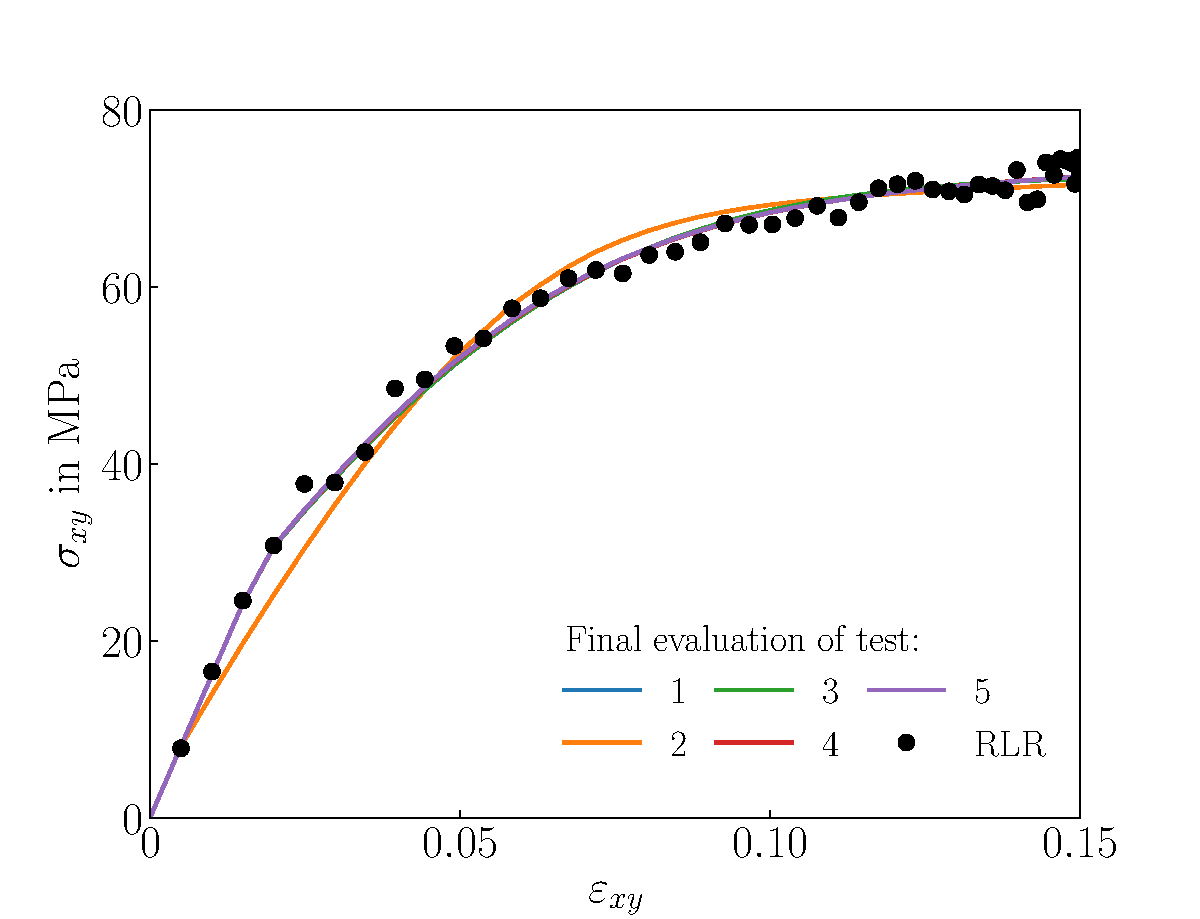
\includegraphics[width=\textwidth]{Shear_6to3_015_fixENu_500_shear_stress_strain.pdf}
        \caption{Final stress-strain curves}
        \label{subfig:shearStressStrain6to3}
\end{subfigure}
\hfill
\begin{subfigure}[t]{0.495\textwidth}
    \centering
    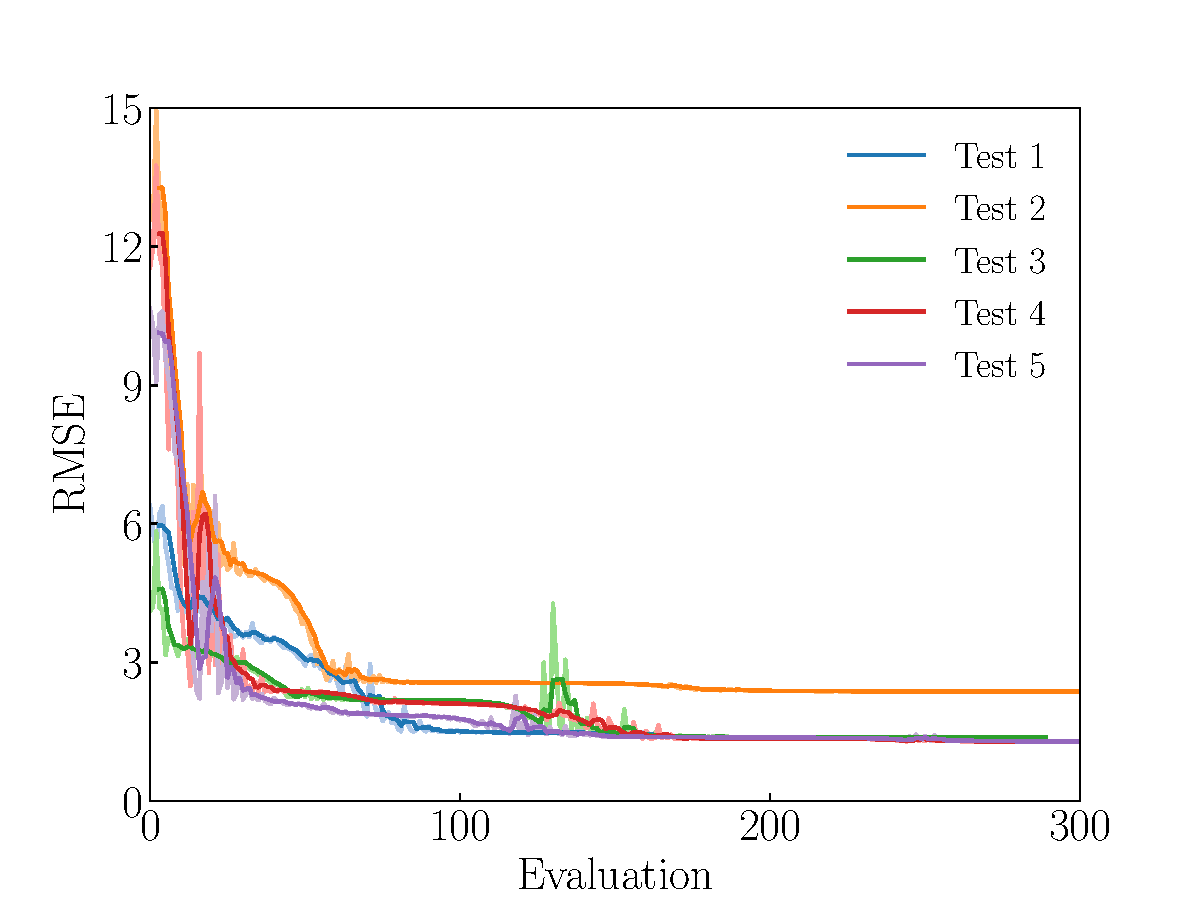
\includegraphics[width=\textwidth]{Shear_6to3_015_fixENu_500_rsme_lin_plot.pdf}
        \caption{ RMSE evolution}
        \label{subfig:shearRMSE}
\end{subfigure}
\caption{Results of shear tests with 6to3 dataset}
\label{fig:shearResults6to3}
\end{figure}

\paragraph{Tensile-Shear combination}

In this test series, the previously presented load cases were combined. Similar, we fixed the elastic parameters before we started the optimisation. However, the defined values for $E$ and $\nu$ must represent the elastic behaviour for both load cases. A comparison of the values we chose in the separate tests shows a high variation. XXX WARUM 
We defined the values as the ones for the simple shear series. The plastic parameters, optimised in this test series are summarised in table XXX. The plastic yield runs into its upper limit of 50 MPa in every test. For alpha and beta the script found similar values for all initial value combinations. Gamma runs into its lower limit of zero in 4 out of 5 cases. 

TABELLE MATERIALPARAMETER

\autoref{fig:CombiResults6to3} depicts the \acrlong{olr} $\sigma_{xx}$ for both load cases. For the tensile load case \autoref{subfig:CombiTensileStressStrainCurve} shows high deviations between the \acrlong{rlr} and the \acrlong{olr}. Only the first and the last point of the reference points is matched by the optimisation tests. In between, the optimised stresses are consequently higher than the reference data. In contrast, the optimised shear stresses show a high correlation to the reference stresses. The optimised shear stresses are slightly lower than the reference data. \autoref{fig:combiRMSE} shows the total error of this test series. Qualitatively, the progress of the error is similar to the ones shown before. However, the absolute value of the error is around 12, which is significantly higher than in all the other studies. We observe this behaviour in all tests within this series. 

\begin{figure}[H]
\centering
\begin{subfigure}[t]{0.495\textwidth}
    \centering
    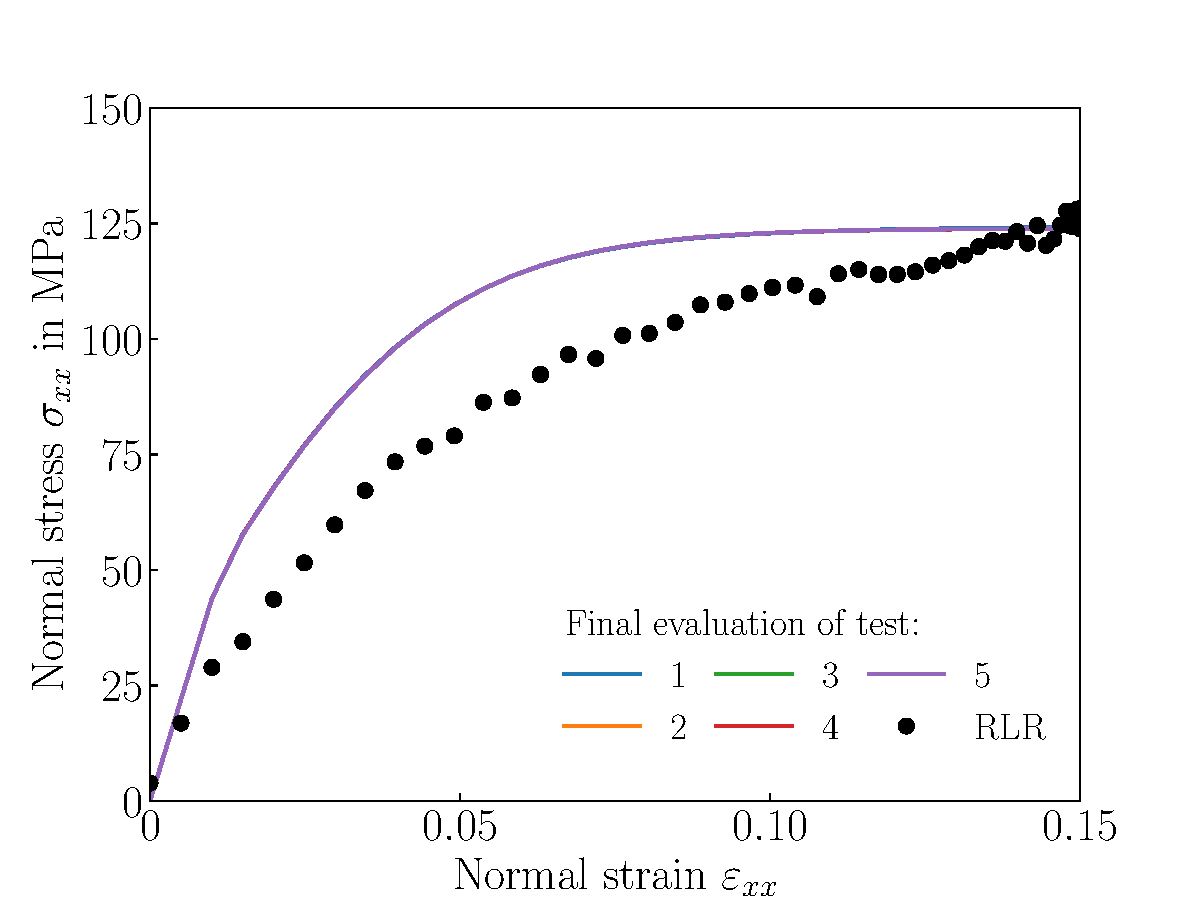
\includegraphics[width=\textwidth]{Combi_6to3_015_fixENu_500a_normal_stress_strain_combined.pdf}
    \caption{Final tensile stress-strain curves}
    \label{subfig:CombiTensileStressStrainCurve}
\end{subfigure}
\hfill
\begin{subfigure}[t]{0.495\textwidth}
    \centering
    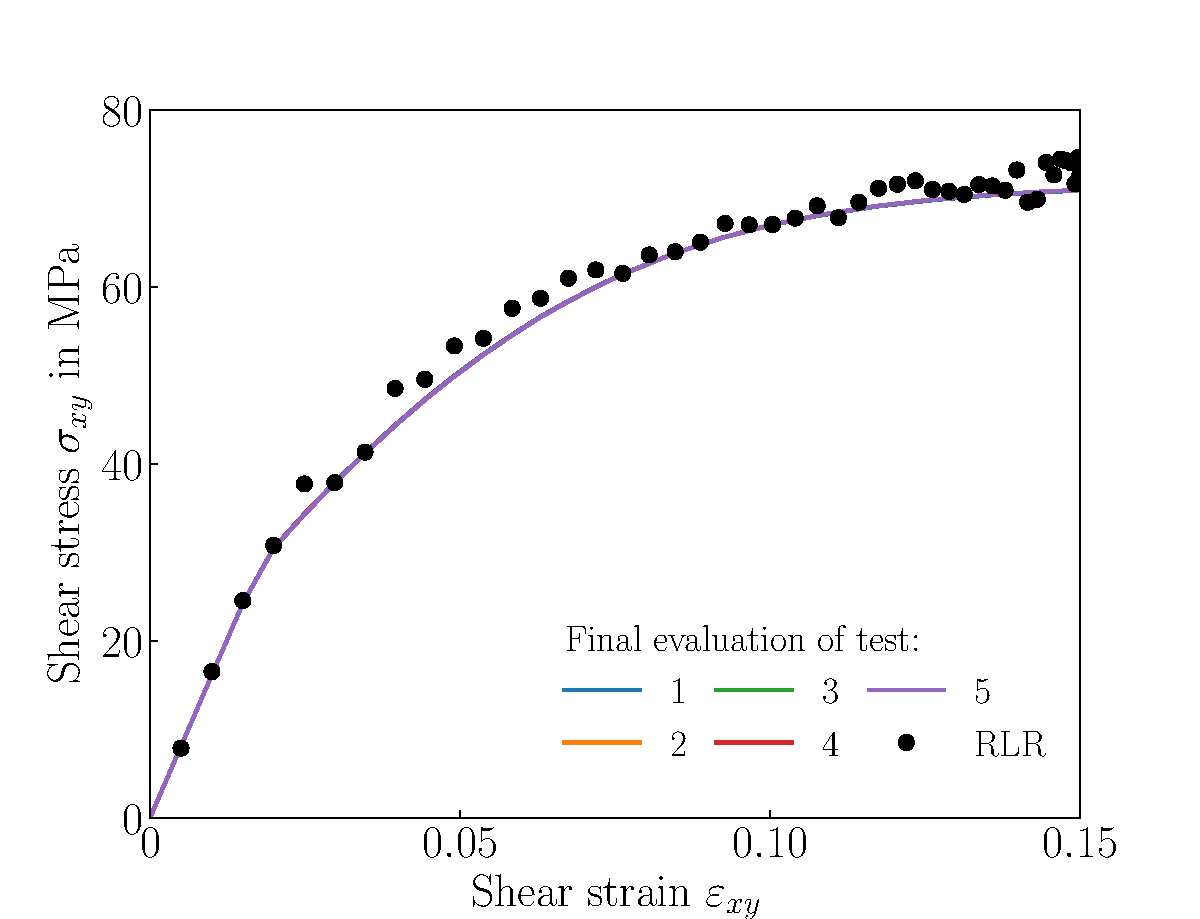
\includegraphics[width=\textwidth]{Combi_6to3_015_fixENu_500a_shear_stress_strain.pdf}
    \caption{Final shear stress strain}
    \label{subfig:CombiShearStressStrain}
\end{subfigure}
\caption{Results of combi tests with 6to3 dataset}
\label{fig:CombiResults6to3}
\end{figure}

\begin{figure}[H]
    \centering
    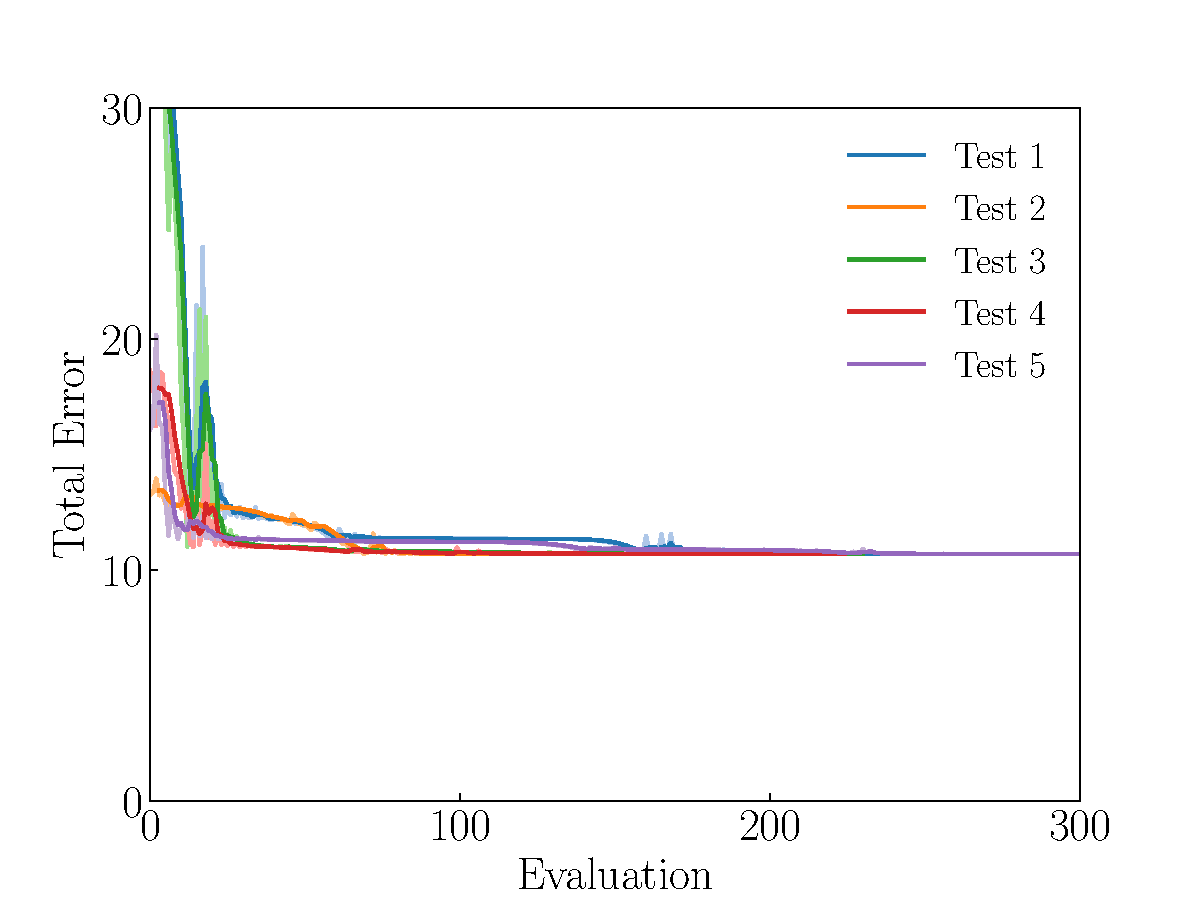
\includegraphics[width=0.495\textwidth]{Combi_6to3_015_fixENu_500a_rsme.pdf}
    \caption{RMSE Combi tests}
    \label{fig:combiRMSE}
\end{figure}

\paragraph{Discussion}
The recently presented results expose some properties of the optmiation script, which need to be discussed. The tensile load case showed similar behaviour as the validation tests. The material parameters $\sigma_0$, $\alpha$ and $\beta$ were determined uniquely, which lead to adequate stress-strain curves. In contrast to the \acrshort{rmse} of the validation results, the \acrshort{rmse} in this study converges at a higher value. This could be explained through the different reference data, used for the studies. In the sinusoidal data set, used in the tensile data set, much more data points are included (see XXX). Therefore, more deviations are possible, which leads to a higher absolute error. Especially, at the end of the loading process, the data become frequent, which makes it impossible to match all with a continuous function. \\
The tests for the simple shear load case show in the load reactions similar results. The \acrlong{olr} match the reference data as good as possible with this frequent number of data points. However, test number 2 behaves like an outlier. Looking at the material parameters (see XX), this behaviour becomes understandable. There, test 2 two hits the lower limit of the plastic yield, and as a Consequence, for alpha and beta different values were determined too. However, in all tests $\sigma_0$ hits one of its limits, which is a behaviour we never saw before in one of the tensile load cases. Therefore, a connection with the new load case of shear load, seems obvious. One possible problem could be the information content of a singular shear test. As \acrlong{er} we only used the corresponding shear stress $\sigma_{xy}$. If this data contain less information, a unique definition of the material parameters is not possible, which is similar to the results of the verification tests (see XX). The value of the plastic yield determines the stress value, where the plastification starts. Difficulties with the definition of this value, could indicate incorrect interpretation of the limit between the elastic and the plastic regime. These problems could occur from the distribution of the reference data in the domains. The ensity of the reference data gets higher with increasing load. Therefore, at the transition from elastic to plastic behaviour, only a few points are given, which restrains a clear separation. In addition, for the definition of the elastic parameters multiple combinations were possibly as described in XX. The influence of different elastic parameters needs additional investigations in some future works, since their impact on the optimisation of the plastic yield is not known so far. Another fact, that could explain difficulties with the shear load case, are the reference data itself. The relaxation procedure, which was used in the \acrshort{md} simulations to eliminate the viscous parts of the stress response, was used only for tensile load applications before. Therefore, the accuracy of this procedure for simple shear is not verified so far. 

Consequently, the optimisation of the remaining plastic parameters, is affect by the behaviour of the plastic yield. Since it hits its limit, the algorotihm has reduced options to optimise the other parameters. Therefore, the similarity of the hardening parameters is a logical consequence of the behaviour of $\sigma_0$. 

In the combined tests, the problems about the shear loading transferred. The plastic yield showed similar behaviour, such that its upper limit was hit in every test. In addition, the elastic parameters computed from the tensile reference data were different from the ones computed from the shear reference data. These two data lead to an insufficient fitting of the tensile load reactions (seeXX). In the tensile stress-strain plot (XX) the slope of the fixed elastic curve is much higher than the reference data, which leads to a higher plastic stress, than the stress in the reference data. Therefore, it is impossible for the script to fit the reference data in the further loading process. We assume the reasons for this inadequate optimisation behaviour in the shear load case. The problems mentioned before, are also valid in combination with other load cases. Therefore, a detailed study about the optimisation behaviour for shear load application is necessary in the future.

NOCH AUF SINUSFÖRMIGES VERHALTNE EINGEHEN   

% - tensile alleine: läuft
% - shear alleine: läuft, aber plasti yield in limit
% - zusammen : läuft nicht
% - problem 1 : elastischen parameter passen nicht zusammen --> warum? 
% --> vlt doch nicht glieches verhalten bei unterschiedlichen belastungen
% --> zu wenige datenpunkte im elastischen bereich 
% --> bei diesen datensätzen unklar, wie lange im elastischen beriech belastet wird--> unklar, mit welchen datenpunkten überhaupt sinnvolle elast parameter berechent werden können


% - problem 2: kurvenform wird fur tensile nicht getroffen 
% --> kurvenformen von zug und scherung passen anscheinend nicht zusammen
% --> oder liegt das daran dass elastische parameter schon falsch sin? 
% --> außerdme unklar ab wann plastifiziert wird -> nachdem plastic yield in schranke gelaufen ist, zeugt das schon von optimierungsproblemen 
% --> vor allem bei der scherung, weil das dort auch shcon einzeln passiert ist 
% --> dort ascheinend schwierig kurve anzunähern ohne in die gernze zu laufen; aber trd ist kurvenfit rel gut; widerspruch 
% --> allg problem, des algortithmus, start der plastifizierung zu bestimmen--> tendenziell wird elastischer bereich als zu groß angenommen bei scherung 

% --> vlt ist problem mit lokalen minima in der funktion 
% --> vlt jz zu viele daten auf einen wert reduziert --> dadurch nimmt gewichtung eines einzelnen datenpunkts ab
% --> vlt bei scherung zu wenig datenpunkte im vorderen bereich (vorgegeben durch md daten); wenn dannn sigma0 nicht gefundne wird, schon verloren
% --> allg einzelner scherversuch vlt zu wening inforamtion um werte zu finen (poisson ratio kannz b eig gar nicht dasraus bestimmt werden --> unbekannt wie diese in den plastischen bereich eingeht); selbst einfluss auf elastischen bereich unbekannt; was wäre, wenn G aus anderen E und nu erzielt worden wäre?
% --> muss auf jedne fall noch weiter untersucht werden
% --> vlt funktioniert relaxationsverfahren für shear tests nicht so gut
% --> andere datensätze in den scherung mit was andere kombiniert wird: liegt das an den datensätzen oder an dem load case?






\section{Cyclic Tests}
IN this section results from tests with cyclic load parameters are presented. We applied a complete sinus period as a tensile load case E11. To gain more information about the elastic behaviour, we combined load parameters with amplitudes of 1\%, 5 \% and 8\% in the optimisation. For this study, the elastic parameters where part of the optimisation, because the values we computed from each data set for $E$ and $\nu$ were different. The material parameters from the final optimisation evaluation are presented in XX for all tests. Each test leads to different material parameters. Beta and Gamma run into their limits in certain tests. 

TABELLE MATWRIALPARAMETER

\begin{figure}[H]
    \centering
    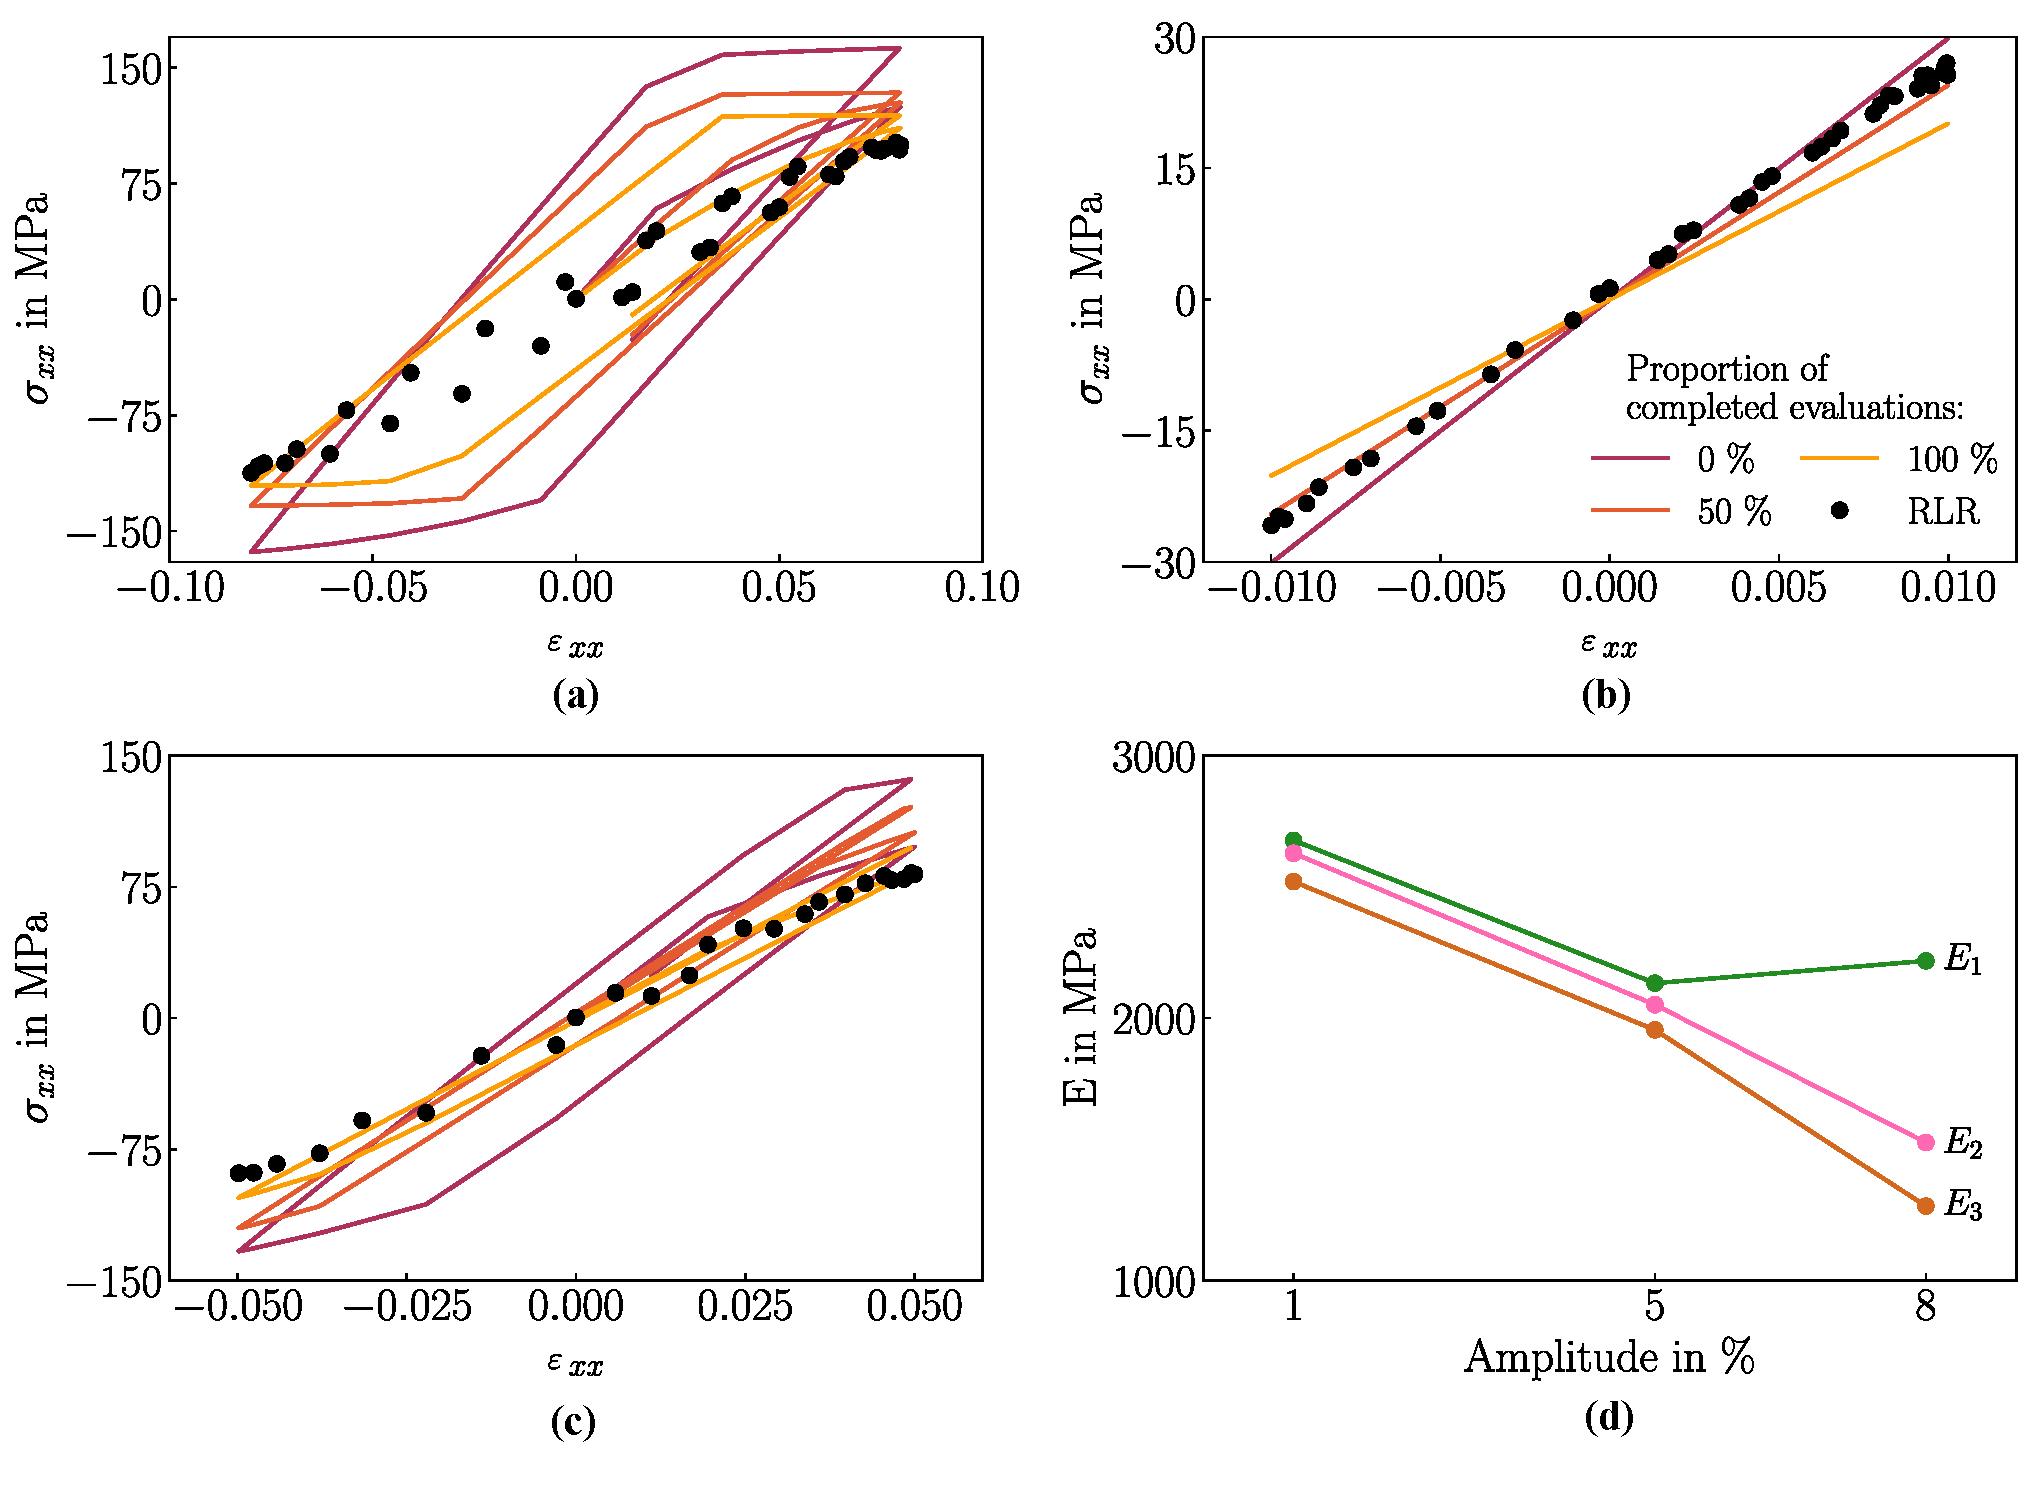
\includegraphics[width=1\textwidth]{combined_cyclic_stress_strain.pdf}
    \caption{Stress Strain plots for 1,5,8 \%}
    \label{fig:cycliclStressStrain}
\end{figure}

To evaluate the quality of the material parameters, we study the \acrlong{olr} $\sigma_{xx}$ for each amplitude in XX. For more clarity, the evolution of the load reactions of each amplitude are plotted separately. In addition, only one exemplary test is shown. A degradation of the match of the \acrlong{rlr} can be observed for the amplitude of 1\%. for the amplitued of 5 adn 8 \% we notice a positive progress during the optimisation run. Especially, in the first rise, both load reactions match adequately with their corresponding reference data. However, during the unloading the error increases for both amplitudes. For 8\% amplitude the deviation is clearly visible. 
\begin{figure}[H]
    \centering
    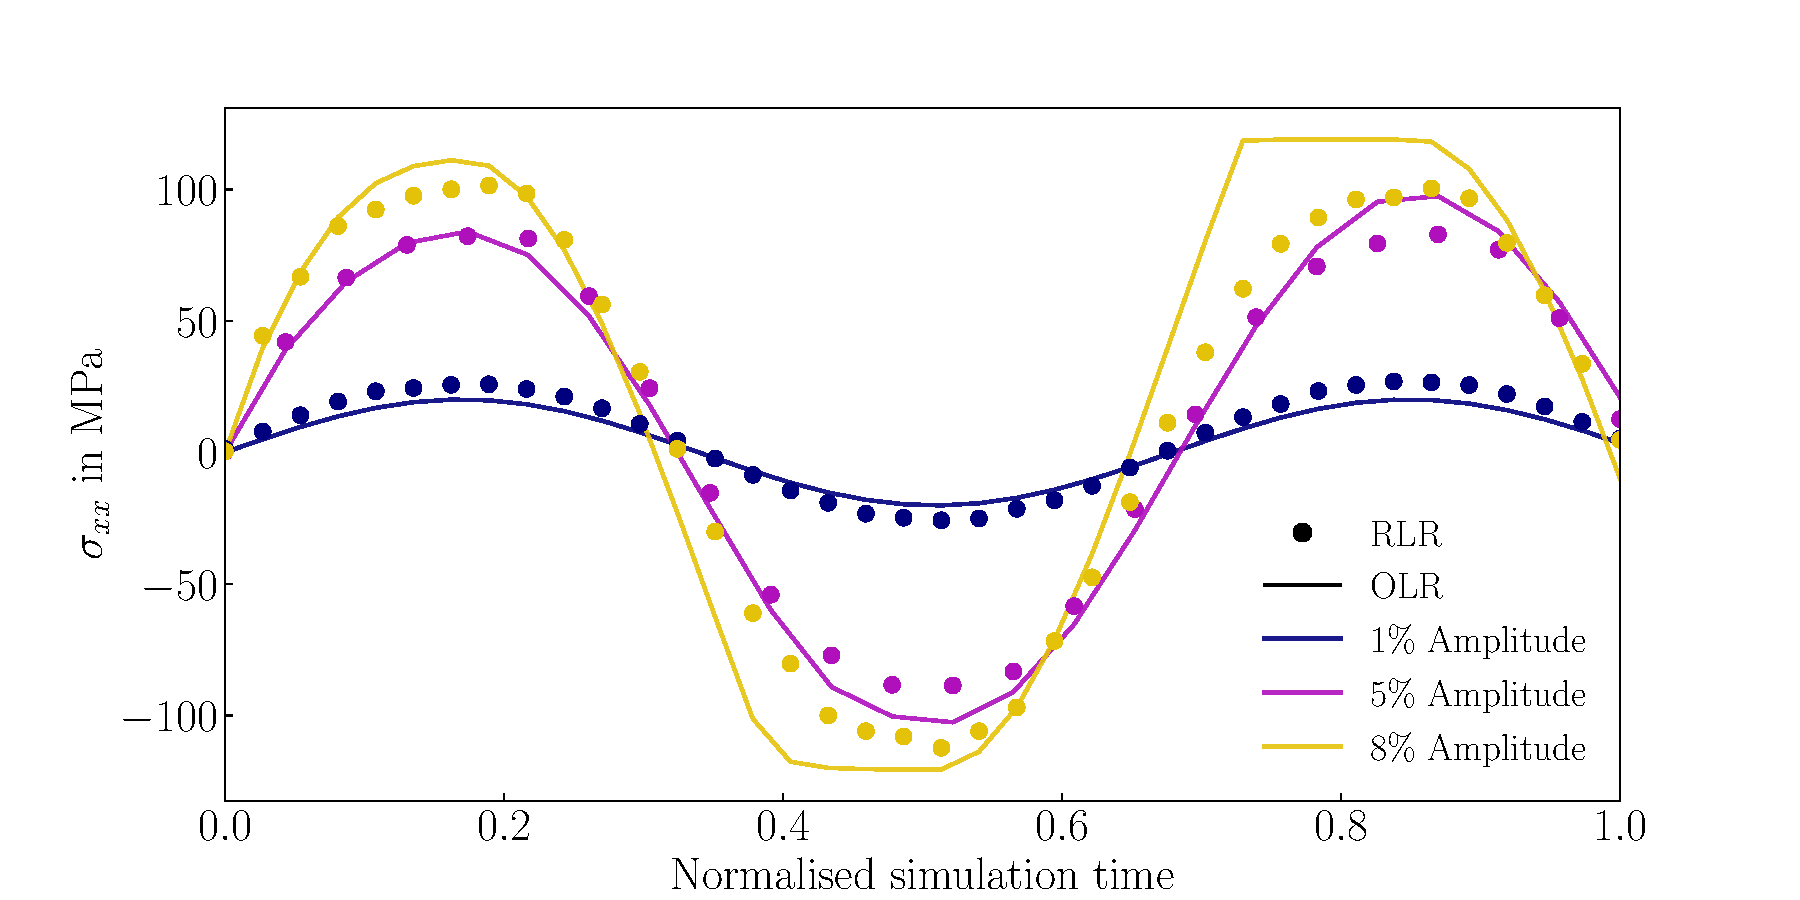
\includegraphics[width=1\textwidth]{CyclicTest_1_5_8Percent_autoInc_4_stress_time.pdf}
    \caption{Stress Time plots for 1,5,8 \%}
    \label{fig:cyclicSterssTime}
\end{figure}

Since the visualization in the stress-strain plot is confusion through the period, we plotted the final load reactions from the same exemplary test over a normalised simulation time in XX. For 1 \% amplitude, the \acrlong{olr} have constantly smaller magnitudes than the reference data. nervertheless, the reference and the optimised data both follow a sinusoidal function during the whole simulation time.  For the other two amplitudes, the data match in the first increasing load steps. During the rest of the loading path, the deviations increase with their maximum values right before or when the maximum stress magnitude is reached. 


RMSE AUSWERTEN

\paragraph{Discussion}
The presented test series gave us additional information about the capabilities of our script. First, the script is able to run an optimisation with three load parameter sets at a time. Since the \acrshort{rmse} decreases, the optmisation principally works. However, the result quality is, measured at the load reactions $\sigma_{xx}$, insufficient. Only the first loading path is adequately depicted with the optmisation. During the negative loading, the deviations increase, which could be explained through changes in the material properties. We assume, that in both cases the plastic regime is reached before the maximum amplitude is reached. Therefore, a hardening process started, which leads to mateiral damage. However, not only the palstic behaviour is influenced. Even in the elastic domain, the slope of the reference curve changes after the first loading sequence. This observation indicates material damage which influences the elastic and the plastic material properties. Since the damage models included in \name{Abaqus} do not handle material damage in the elastic region, a self-written user-subroutine is necessary to depict the damage behaviour. The inclusion of material damage would lead to an improvement of the script to process cyclic load parameters, which should be part of future investigations. 


- drei load paraameter. set auf jeinmal getestet: geht prinzipell
- cyclcic load geht nicht:
- bei 1 % noch am ehesten 
- dort vmtl nur elastisches verhalten, müsste einzeln untersucht werden,ob man das abbilden kann
- die anderen beiden nicht, weil spätestens bei negativer belastung passen olr und rlr nicht merh zusammen --> schäädigung tritt auf, die wir niht abbilden können 
- further invstigations








